%% LyX 2.1.4 created this file.  For more info, see http://www.lyx.org/.
%% Do not edit unless you really know what you are doing.
\documentclass{beamer}
\usepackage{hyperref}
\usepackage{minted}
\usepackage{animate}
\usepackage{graphicx}
\def\Put(#1,#2)#3{\leavevmode\makebox(0,0){\put(#1,#2){#3}}}
\usepackage{color}
\usepackage{tikz}
\usepackage{amssymb}

\newcommand\blfootnote[1]{%
  \begingroup
  \renewcommand\thefootnote{}\footnote{#1}%
  \addtocounter{footnote}{-1}%
  \endgroup
}

\definecolor{LightGray}{gray}{0.9}

\ifx\hypersetup\undefined
  \AtBeginDocument{%
    \hypersetup{unicode=true,
 bookmarksnumbered=false,bookmarksopen=false,
 breaklinks=false,pdfborder={0 0 0},colorlinks=false}
  }
\else
  \hypersetup{unicode=true,
 bookmarksnumbered=false,bookmarksopen=false,
 breaklinks=false,pdfborder={0 0 0},colorlinks=false}
\fi

\makeatletter
%%%%%%%%%%%%%%%%%%%%%%%%%%%%%% Textclass specific LaTeX commands.
 % this default might be overridden by plain title style
 \newcommand\makebeamertitle{\frame{\maketitle}}%
 % (ERT) argument for the TOC
 \AtBeginDocument{%
   \let\origtableofcontents=\tableofcontents
   \def\tableofcontents{\@ifnextchar[{\origtableofcontents}{\gobbletableofcontents}}
   \def\gobbletableofcontents#1{\origtableofcontents}
 }

%%%%%%%%%%%%%%%%%%%%%%%%%%%%%% User specified LaTeX commands.
\usetheme{Malmoe}
% or ...
\useoutertheme{infolines}
\addtobeamertemplate{headline}{}{\vskip2pt}

\setbeamercovered{transparent}
% or whatever (possibly just delete it)



\setbeamertemplate{footline}
{
  \leavevmode%
  \hbox{%
  \begin{beamercolorbox}[wd=.5\paperwidth,ht=2.25ex,dp=1ex,center]{title in head/foot}%
    \usebeamerfont{title in head/foot}\insertshorttitle
  \end{beamercolorbox}%
  \begin{beamercolorbox}[wd=.5\paperwidth,ht=2.25ex,dp=1ex,right]{date in head/foot}%
    \usebeamerfont{date in head/foot}\insertshortdate{}\hspace*{2em}
    \insertframenumber{} / \inserttotalframenumber\hspace*{2ex} 
  \end{beamercolorbox}}%
  \vskip0pt%
}

\makeatother

\begin{document}

\title[Qualification]{Towards Parallel Detection of Movement Patterns in Large Spatio-temporal Datasets}
\subtitle{Oral Qualification}
\author{Andres Calderon}
%\institute{University of California, Riverside}

\makebeamertitle

% \AtBeginSection[]{
%   \frame<beamer>{ 
%     \frametitle{Agenda}   
%     \tableofcontents[currentsubsection] 
%   }
% }

\newif\iflattersubsect

\AtBeginSection[] {
    \begin{frame}<beamer>
    \frametitle{Outline} %
    \tableofcontents[currentsection]  
    \end{frame}
    \lattersubsectfalse
}

\AtBeginSubsection[] {
    % \iflattersubsect
    \begin{frame}<beamer>
    \frametitle{Outline} %
    \tableofcontents[currentsubsection]  
    \end{frame}
    % \fi
    % \lattersubsecttrue
}

\section*{Introduction}

\begin{frame}{Trajectory datasets}
  \begin{itemize}
    \item Anything that could move (or could be moved), will be tracked...
    \begin{itemize}
      \item Sensors, Sensors everywhere...
      \item Smart phones, GPS, RFID, WiFi, Bluetooth, ZigBee, IoT, Satellites, Drones, Surveillance cameras...
    \end{itemize}
  \end{itemize}
\end{frame}

\begin{frame}{Applications}
  Tracking social behavior of animal colonies.
  \centering
  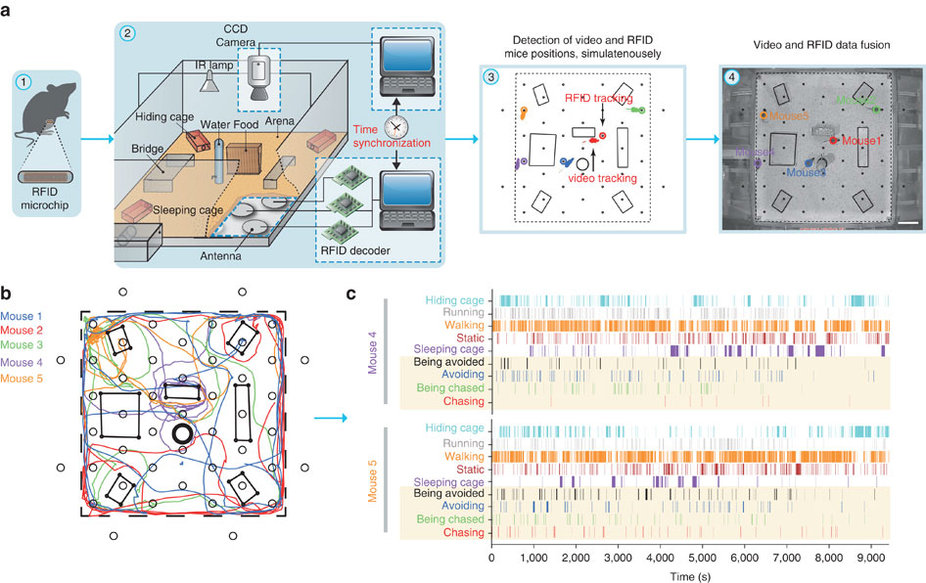
\includegraphics[width=0.85\linewidth]{Figures/mouse.jpg}
  \blfootnote{\tiny  \href{http://tinyurl.com/jjfqmhh}{(Weissbrod et al, Nature'13)}}
\end{frame}

\begin{frame}{Applications}
  Are you a returner or an explorer? Ask Big Data.
  \centering
  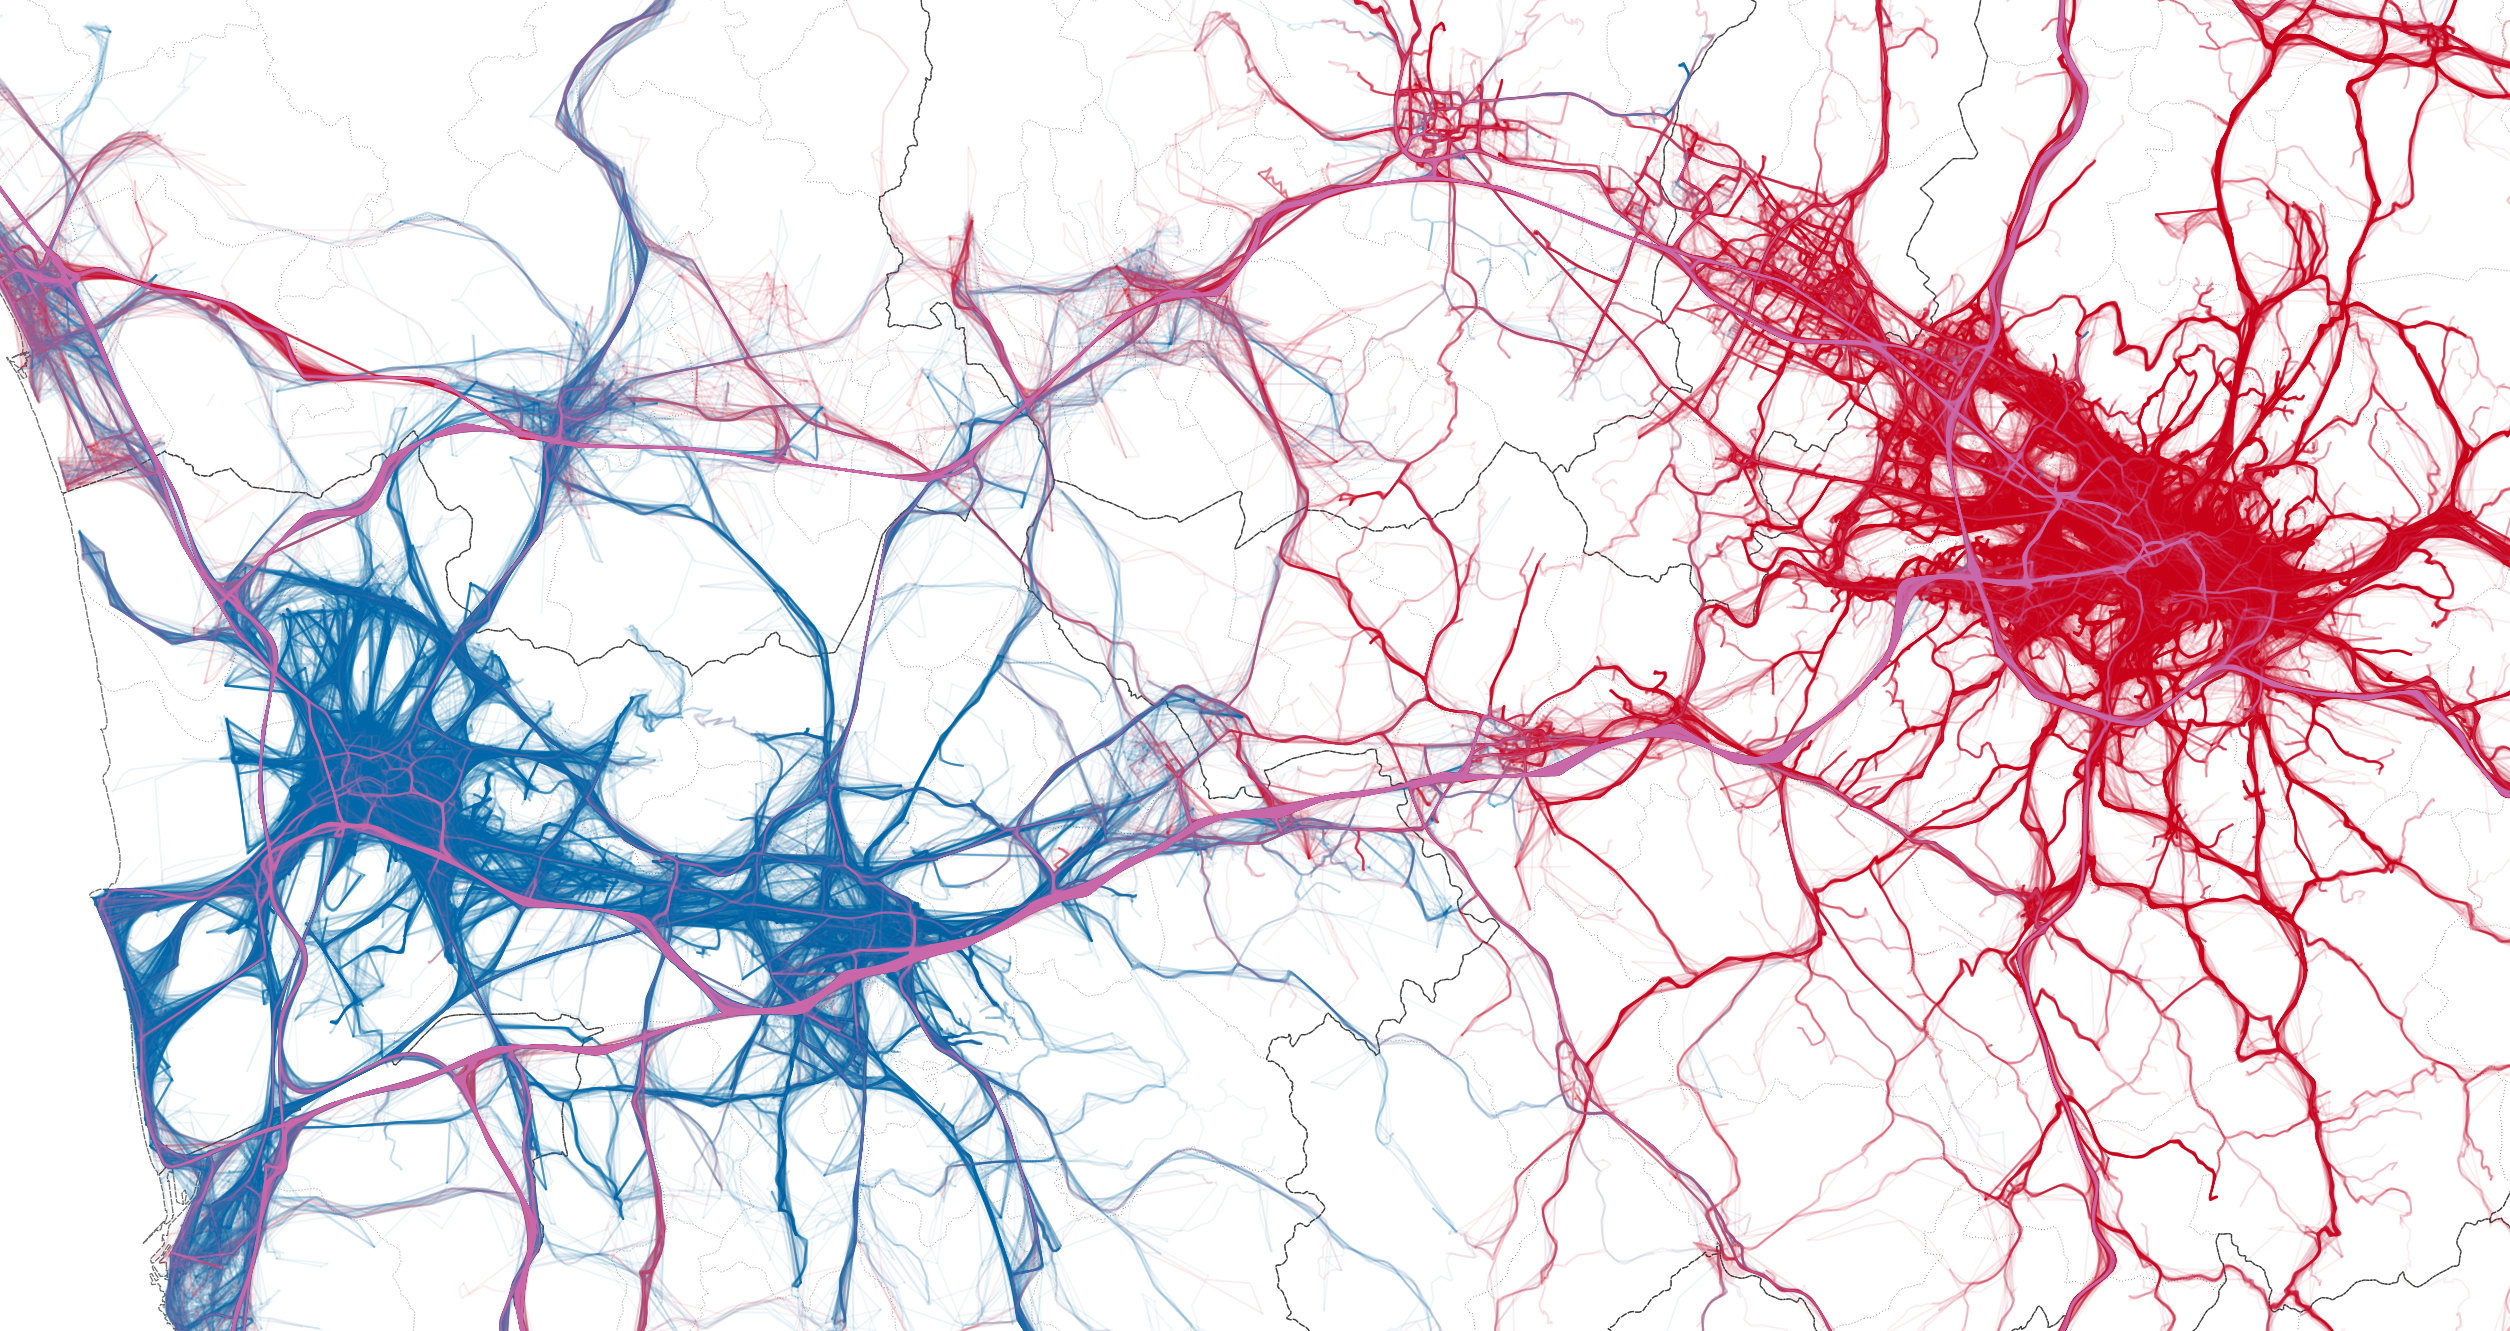
\includegraphics[width=\linewidth]{Figures/roe.png}
  \blfootnote{\tiny \href{https://tinyurl.com/m54xmm4}{(Pappalardo et al, Nature'15)}}
\end{frame}

\begin{frame}{}
  Tiger shark data analysis.
  \centering
  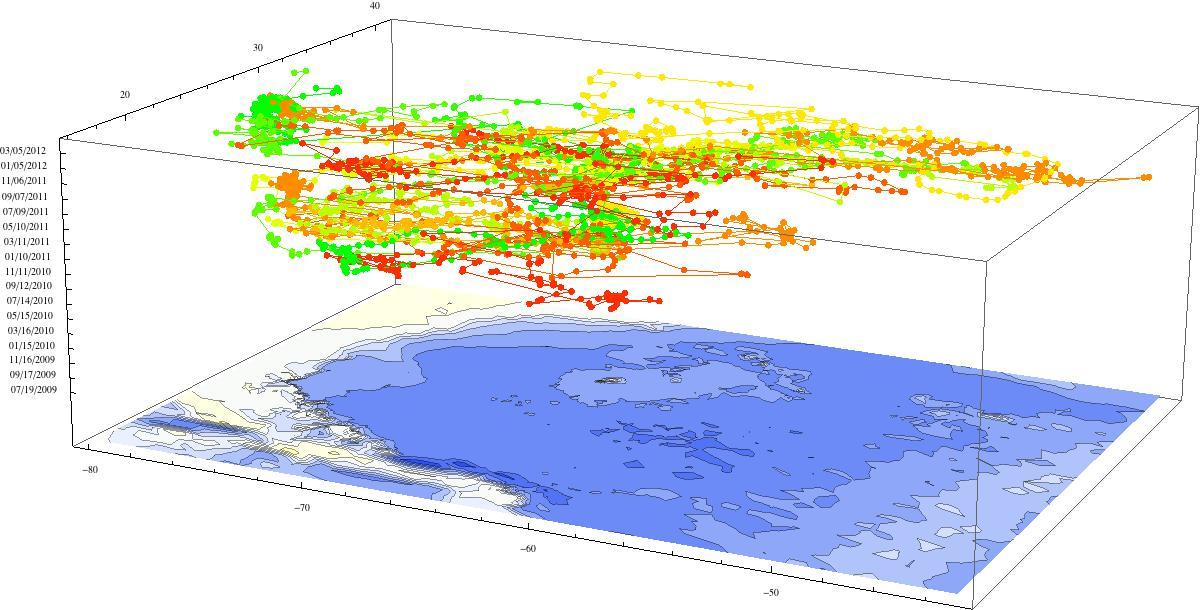
\includegraphics[width=\linewidth]{Figures/sharks.jpg}
  \blfootnote{\tiny \href{http://tinyurl.com/gtqjh4o}{(Antonov, 2012)}}
\end{frame}

\begin{frame}{Applications}
  Visual mining of cyclone paths.
  \centering
  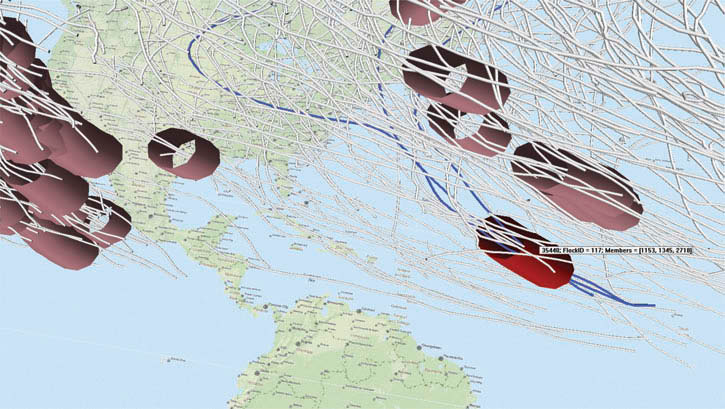
\includegraphics[width=.85\linewidth]{Figures/cyclones.png}
  \blfootnote{\tiny \href{https://tinyurl.com/nhmwerr}{(Turdukulov, IJGIS'14)}}
\end{frame}

\begin{frame}{Applications}
  Bird migration forecast.
  \centering
  \animategraphics[autoplay, loop,width=1\textheight]{5}{Figures/birds2/frame-}{0}{51}
  \blfootnote{\tiny \href{http://ebird.org/content/ebird/occurrence/}{(Sullivan et al, Biological Conservation'14)}}
\end{frame}

\begin{frame}{Complex movement patterns}
 Previous works focus on traditional queries:
 \begin{itemize}
  \item Range
  \item Nearest Neighbors
  \item Similarity
 \end{itemize}
 \centering 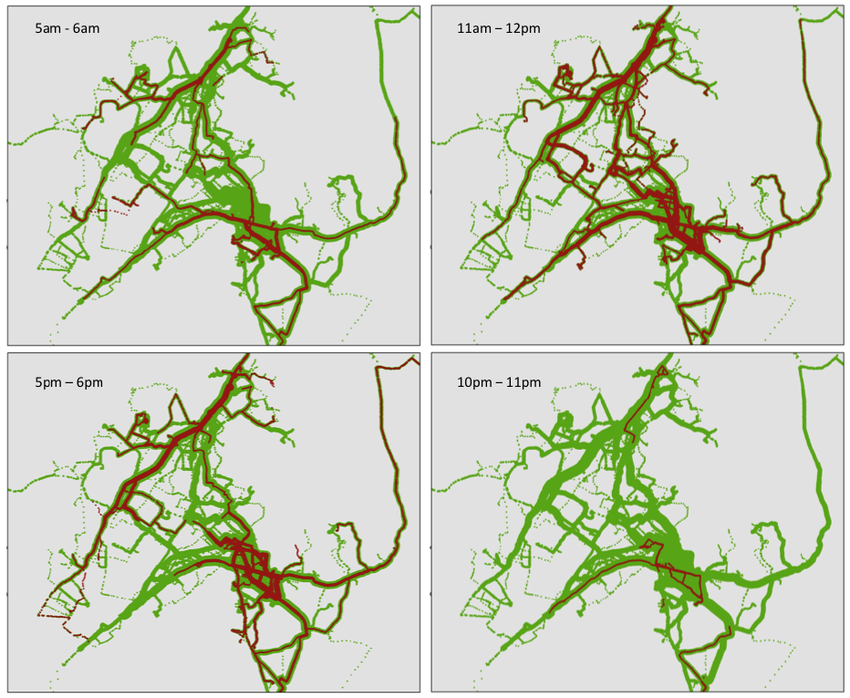
\includegraphics[height=0.5\textheight]{Figures/similarity.png}
\end{frame}

\begin{frame}{Complex movement patterns}
  Recent works look for the aggregate behavior:\vspace{2mm}
  \begin{minipage}{.5\textwidth}
    \begin{itemize}
    \item Moving clusters
    \item Convoys
    \item Flocks
    \item Swarms
    \item Gatherings
    \end{itemize}
  \end{minipage}\begin{minipage}{.5\textwidth}
    \centering 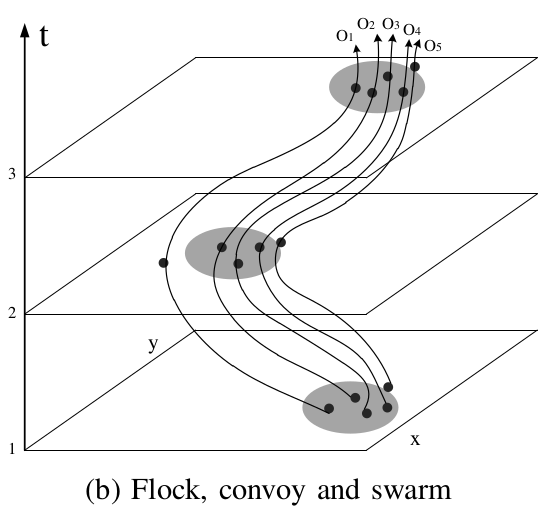
\includegraphics[width=0.5\textwidth]{Figures/cmp1.png}\\
    \centering 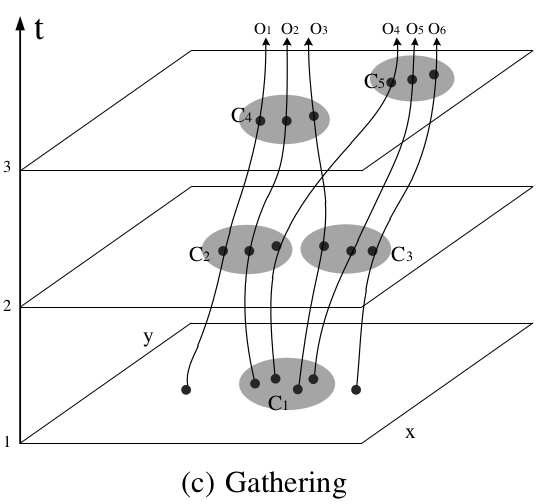
\includegraphics[width=0.5\textwidth]{Figures/cmp2.png}
    \begin{flushright}
     \tiny (Zheng et al, ICDE'13)
    \end{flushright}
  \end{minipage}
\end{frame}

\begin{frame}{Complex movement patterns}
  Recent works look for the aggregate behavior:\vspace{2mm}
  \begin{minipage}{.5\textwidth}
    \begin{itemize}
    \item Moving clusters
    \item Convoys
    \item \textbf{Flocks}
    \item Swarms
    \item Gatherings
    \end{itemize}
  \end{minipage}\begin{minipage}{.5\textwidth}
    \centering 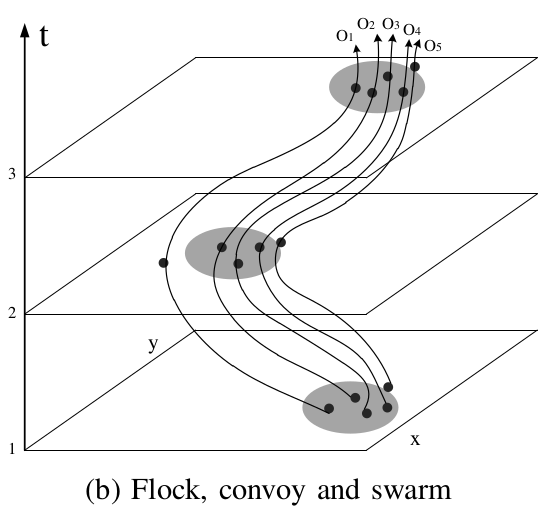
\includegraphics[width=0.5\textwidth]{Figures/cmp1.png}\\
    \centering 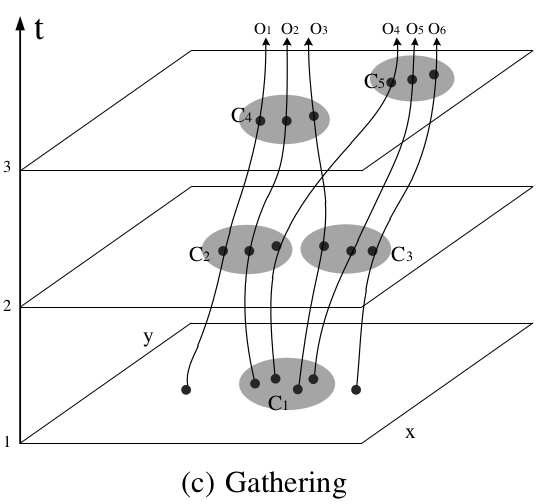
\includegraphics[width=0.5\textwidth]{Figures/cmp2.png}
    \begin{flushright}
     \tiny (Zheng et al, ICDE'13)
    \end{flushright}
  \end{minipage}
\end{frame}

\section{Moving flock patterns}

\begin{frame}{What is a flock???} 
  \begin{definition}[$(\mu,\epsilon,\delta)-flock$]
    Sets of at least \alert{ $\mu$ } objects moving close enough (\alert{ $\varepsilon$ }) for at least \alert{ $\delta$ } time intervals \tiny (Benkert et al, 2008). 
  \end{definition}
  \centering 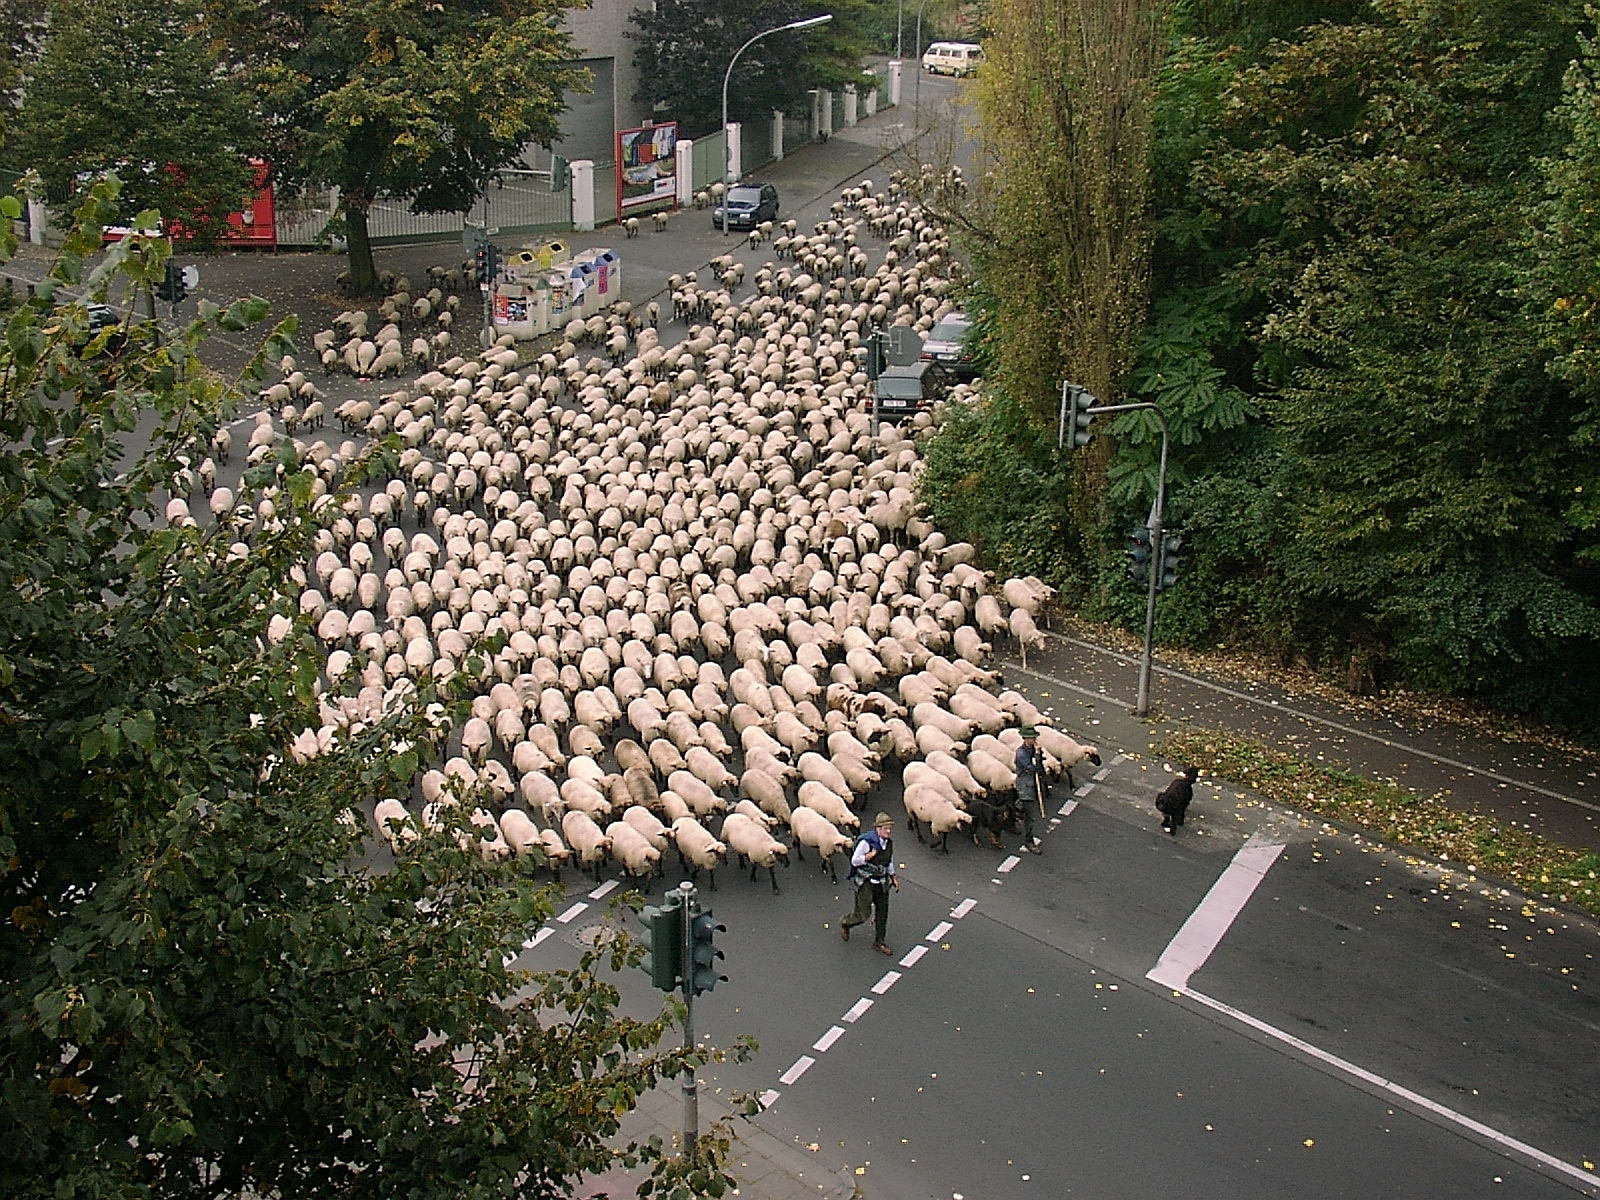
\includegraphics[height=0.6\textheight]{Figures/flock2.jpg}
\end{frame}

\begin{frame}{BFE algorithm \tiny (Vieira et al, 2009)}
  \centering 
\includegraphics[page=2,height=0.7\textheight]{Figures/flock/f0}
\end{frame}
\begin{frame}[noframenumbering]{BFE algorithm \tiny (Vieira et al, 2009)}
  \centering 
\includegraphics[page=2,height=0.7\textheight]{Figures/flock/f1}
\end{frame}
\begin{frame}[noframenumbering]{BFE algorithm \tiny (Vieira et al, 2009)}
  \centering 
\includegraphics[page=2,height=0.7\textheight]{Figures/flock/f3}
\end{frame}
\begin{frame}[noframenumbering]{BFE algorithm \tiny (Vieira et al, 2009)}
  \centering 
\includegraphics[page=2,height=0.7\textheight]{Figures/flock/f4}
\end{frame}
\begin{frame}[noframenumbering]{BFE algorithm \tiny (Vieira et al, 2009)}
  \centering 
\includegraphics[page=2,height=0.7\textheight]{Figures/flock/f5}
\end{frame}
\begin{frame}[noframenumbering]{BFE algorithm \tiny (Vieira et al, 2009)}
  \centering 
\includegraphics[page=2,height=0.7\textheight]{Figures/flock/f7}
\end{frame}
\begin{frame}[noframenumbering]{BFE algorithm \tiny (Vieira et al, 2009)}
  \centering 
\includegraphics[page=2,height=0.7\textheight]{Figures/flock/f8}
\end{frame}
\begin{frame}[noframenumbering]{BFE algorithm \tiny (Vieira et al, 2009)}
  \centering 
\includegraphics[page=2,height=0.7\textheight]{Figures/flock/f9}
\end{frame}
\begin{frame}[noframenumbering]{BFE algorithm \tiny (Vieira et al, 2009)}
  \centering 
\includegraphics[page=2,height=0.7\textheight]{Figures/flock/f10}
\end{frame}

\begin{frame}{Motivation}
  Why is important to focus on flocks and finding disks???
  \begin{itemize}
    \item Why are moving flock patterns important?
    \begin{itemize}
      \item They capture the collective behavior of trajectories as groups.
      \item A general model for other movement patterns.
    \end{itemize}
    \item Why is the finding of disks important?
    \begin{itemize}
      \item It is no trivial, disks can be at any location.      
      \item It has a high complexity ($\mathcal{O}(2n^2)$).
      \item Number of disks can be huge and it can require further filtering.
    \end{itemize}
  \end{itemize}
\end{frame}

\begin{frame}{Contributions}
  This work focuses on improvements in the two initial parts of the BFE algorithm:
  \begin{enumerate}
   \item Boost the detection of a candidate set of disks through a parallel approach.
   \item Apply a frequent pattern approach in order to improve the filtering of disks.
  \end{enumerate}
\end{frame}

\section{Finding candidate disks}
\subsection{Implementation}

\begin{frame}{BFE implementation}
    \begin{itemize}
     \item On-Line Discovery of Flock Patterns in Spatio-Temporal Data \tiny (Vieira et al, SIGSPATIAL'09).
     \item \normalsize Implementation available at \url{https://github.com/poldrosky/FPFlock}.
    \end{itemize}
\end{frame}

\begin{frame}{BFE implementation}
 \centering
 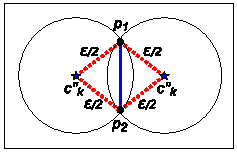
\includegraphics[width=0.5\textwidth]{Figures/theorem} 
\end{frame}

\begin{frame}{BFE implementation}
 \centering
 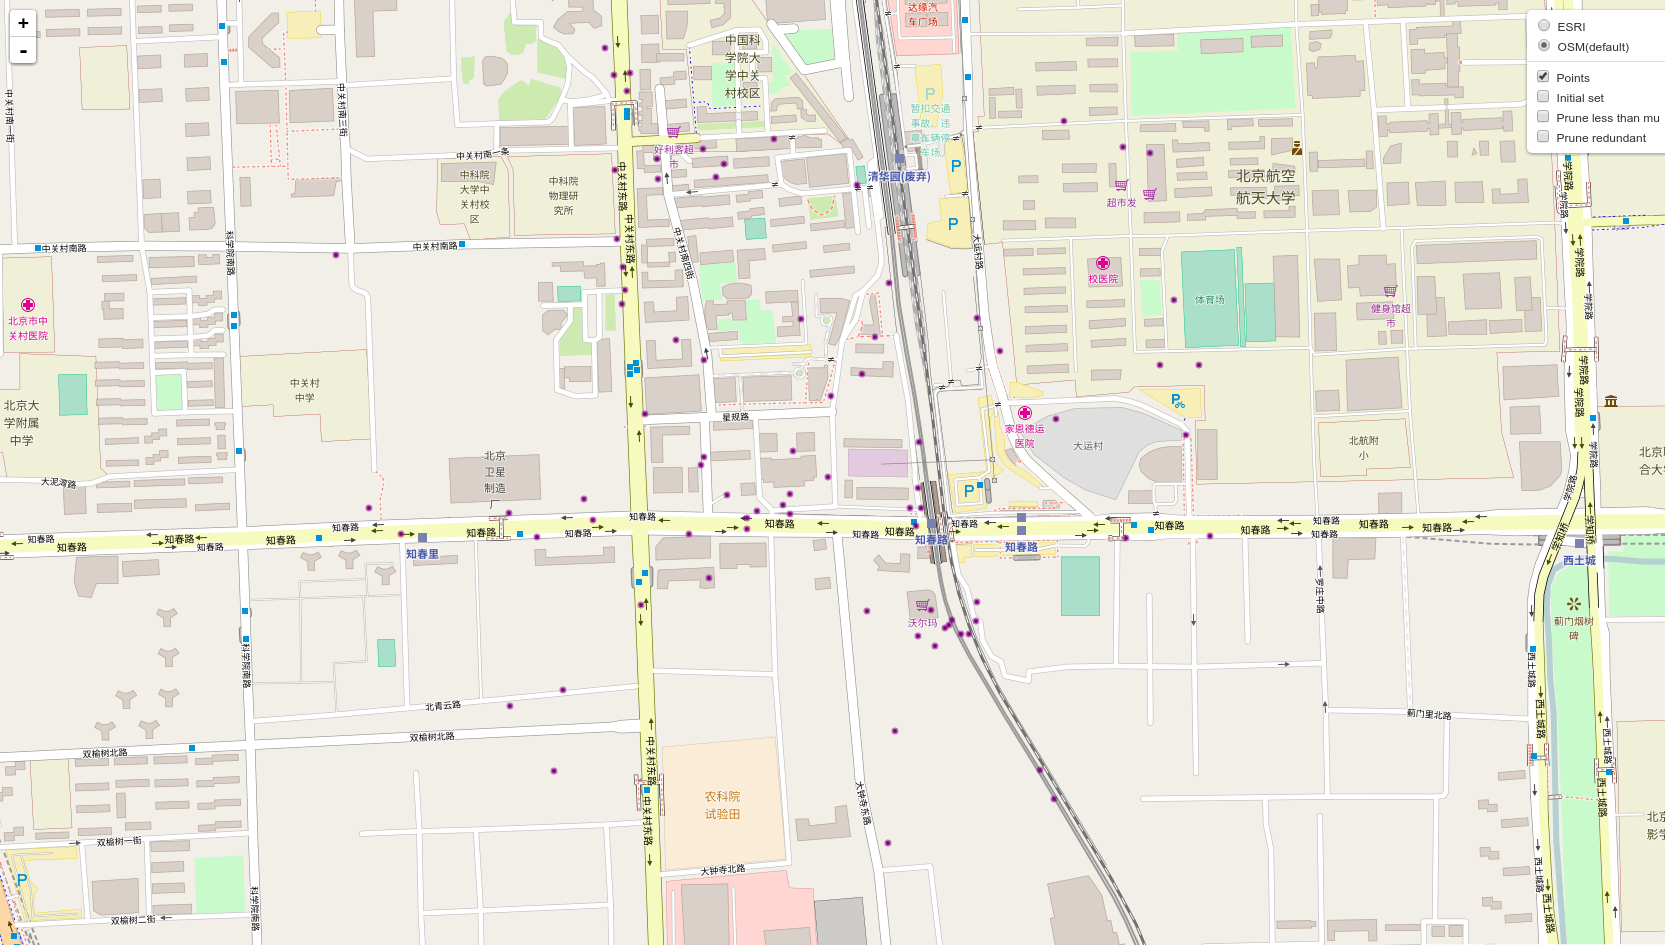
\includegraphics[trim={5cm 3cm 5cm 0}, clip, width=\textwidth]{Figures/d01.png} 
\end{frame}
\begin{frame}[noframenumbering]{BFE implementation}
 \centering
 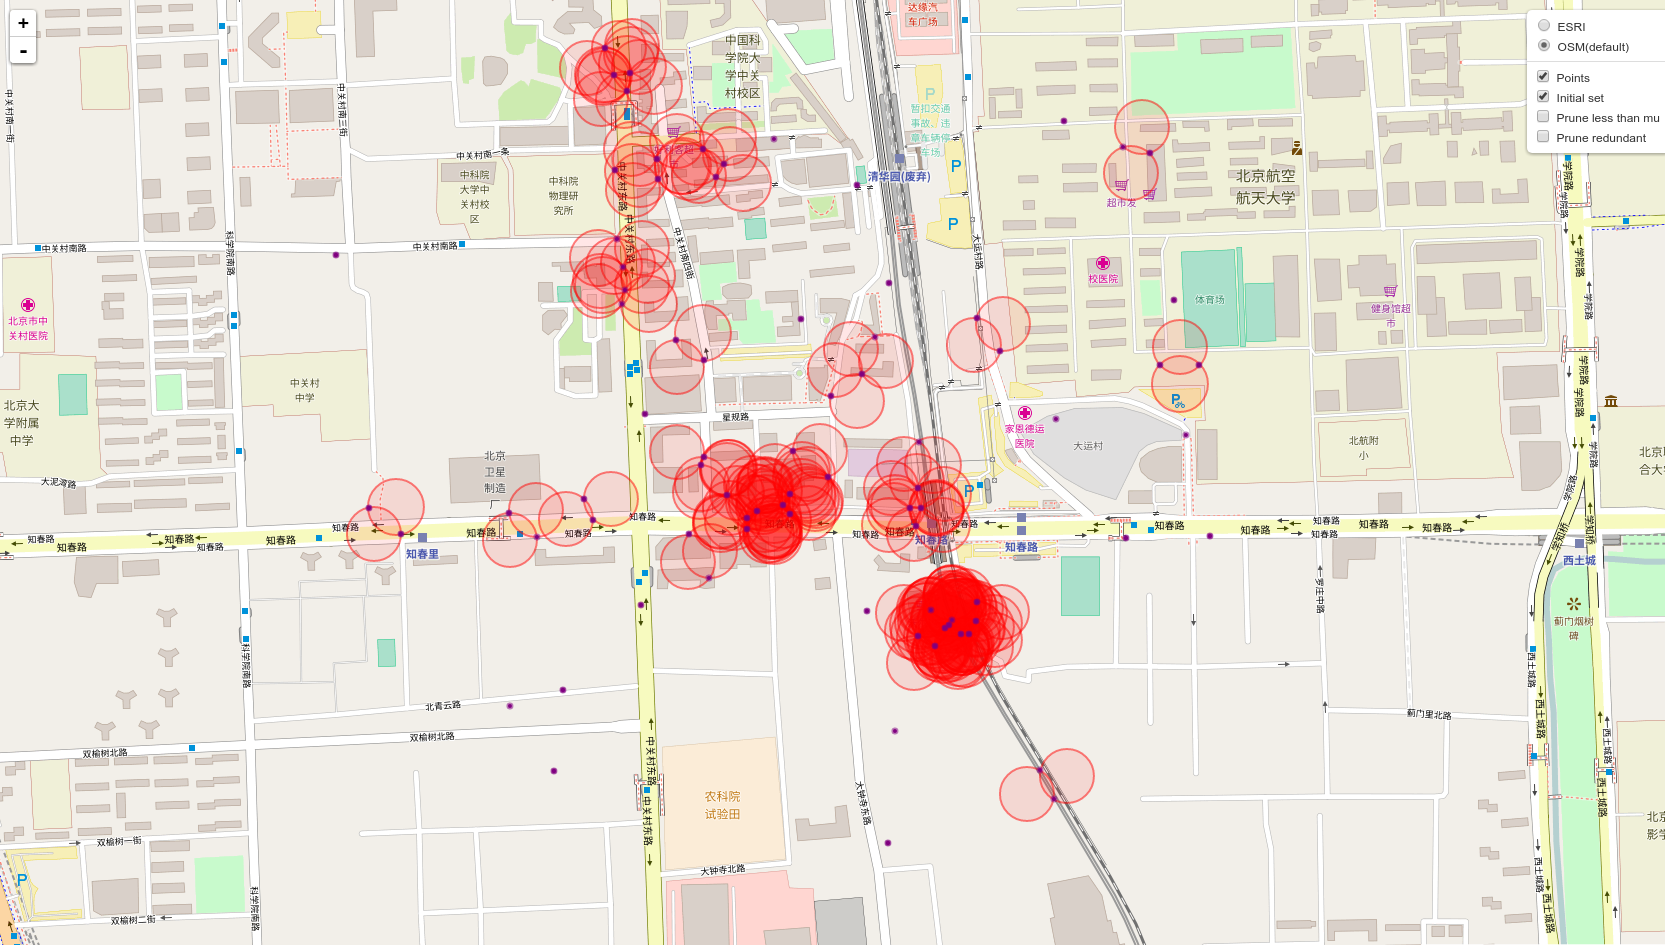
\includegraphics[trim={5cm 3cm 5cm 0}, clip, width=\textwidth]{Figures/d02.png} 
\end{frame}

\begin{frame}{PBFE implementation}
    \begin{itemize}
     \item Written in Scala using Simba 1.6.3.
     \begin{itemize}
      \item Tested by visual inspection and counting number of found disks.
     \end{itemize}
	\item Code available at \\ \scriptsize \url{https://github.com/aocalderon/PhD/tree/master/Y2Q1/SDB/Project/Code/Scripts/pbfe2}.
    \end{itemize}
\end{frame}

\begin{frame}{PBFE implementation}
    \begin{itemize}
     \item Simba (Xie et al, SIGMOD'16) provides rich spatial operations through both SQL and the DataFrame API.
     \item Two-layer spatial indexing, cost-based optimization, open source.
     \item \texttt{DISTANCE JOIN} and \texttt{CIRCLERANGE} operators were the key!!!
    \end{itemize}
\end{frame}

\begin{frame}[fragile]{PBFE implementation}
	\begin{minted}[fontsize=\tiny,tabsize=8,breaklines,framesep=10pt,frame=single, escapeinside=||,mathescape=true]{sql}
		SELECT 
			*
		FROM 
			points p1
		|\color{blue}{DISTANCE JOIN}|
			points p2 
		ON 
			POINT(p2.x, p2.y) IN |\color{blue}{CIRCLERANGE}|(POINT(p1.x, p1.y), |$\varepsilon$|)
		WHERE 
			p1.id < p2.id
	\end{minted}
	\vspace{1mm}
 \centering
 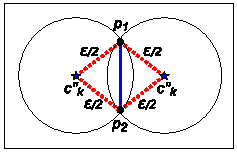
\includegraphics[width=0.3\textwidth]{Figures/theorem} 
\end{frame}

\subsection{Experiments}

\begin{frame}{Dataset}
  \begin{itemize}
    \item \textbf{Beijing} from Geolife project\footnote{\tiny \url{http://tinyurl.com/j7t2cao}}.
    \begin{itemize}
     \item 182 users in a period of over three years (from April 2007 to August 2012).
     \item 17,621 trajectories.
     \item $\approx$18 million points (no duplicates).
    \end{itemize}
  \end{itemize}
\end{frame}

\begin{frame}{Beijing dataset}
  \centering
  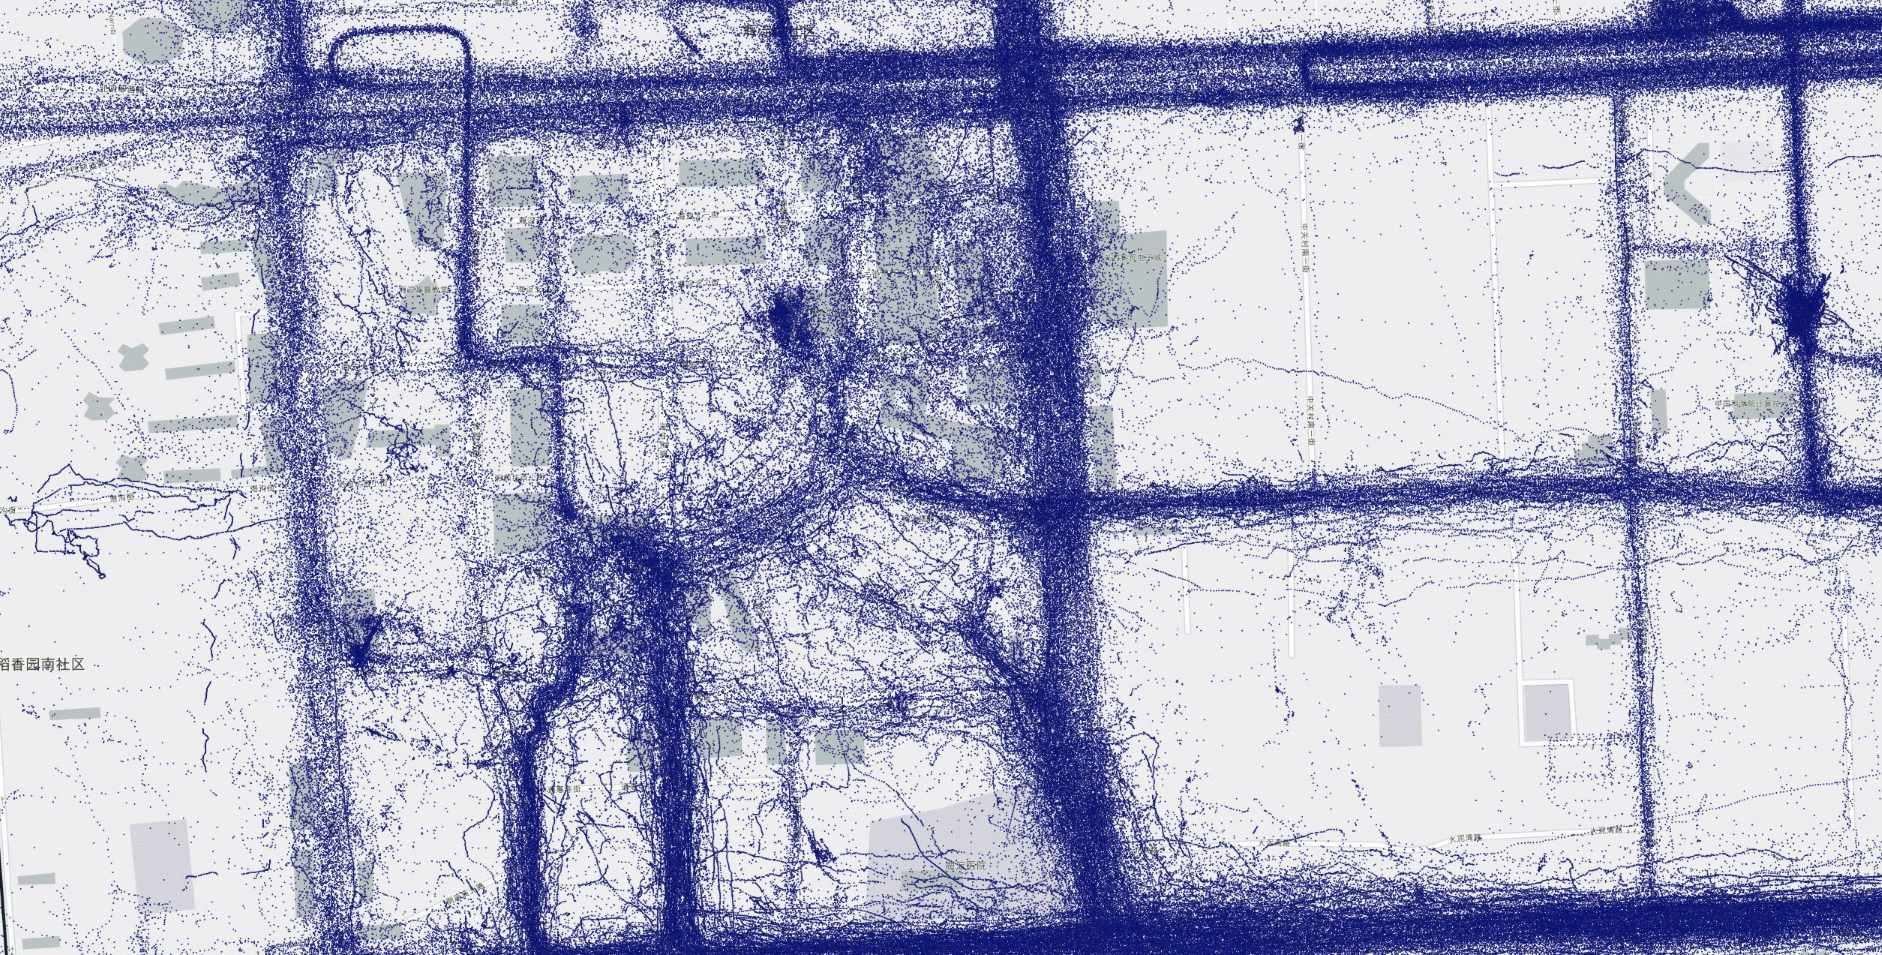
\includegraphics[width=\textwidth]{Figures/geolife.jpg}
\end{frame}

\begin{frame}{Setup}
  \begin{itemize}
    \item Single-node.
    \item Processor: 4-core Intel(R) Core(TM) i5-2400S CPU @ 2.50GHz
    \item RAM: 8 GB.
    \item Ubuntu 16.04 LTS, Simba/Spark 1.6.3.
  \end{itemize}
\end{frame}

\begin{frame}{Execution time}
  \centering
  \href{http://www.cs.ucr.edu/~acald013/public/Beijing10K-100K_E10-200_animation.gif}{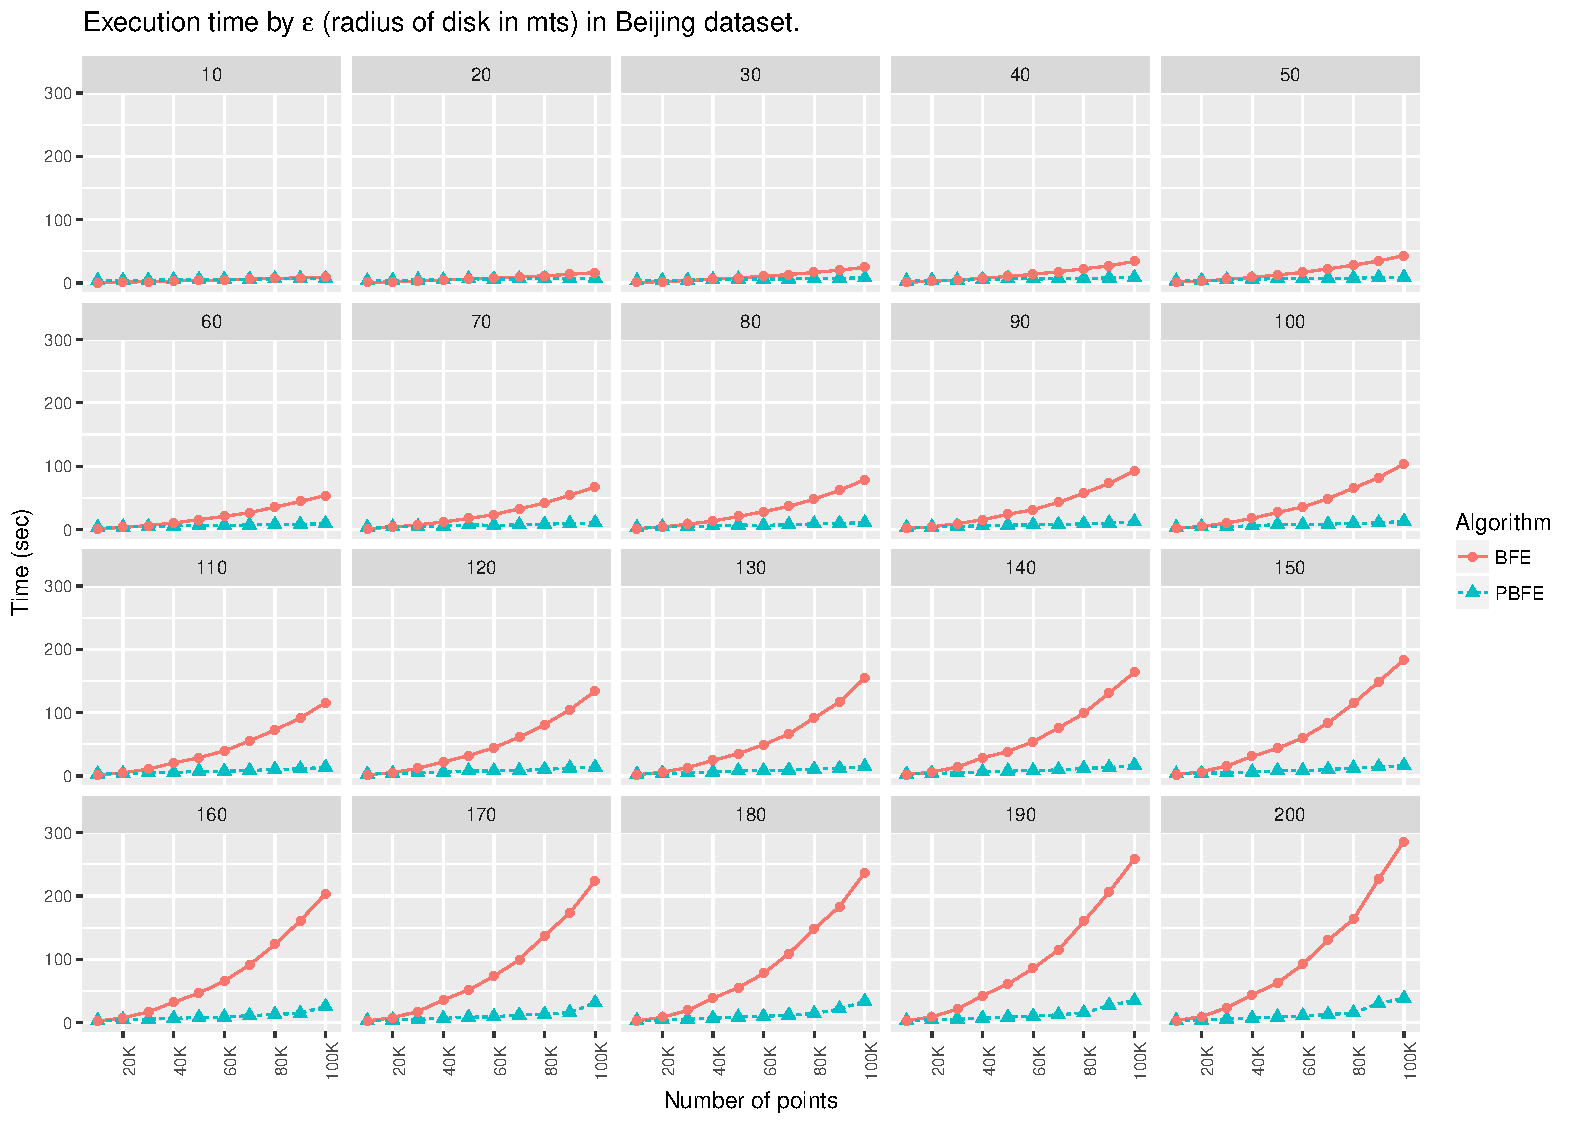
\includegraphics[height=0.85\textheight]{Figures/Beijing10K-100K_E10-200}}
\end{frame}

\begin{frame}{Scaleup}
  \centering
  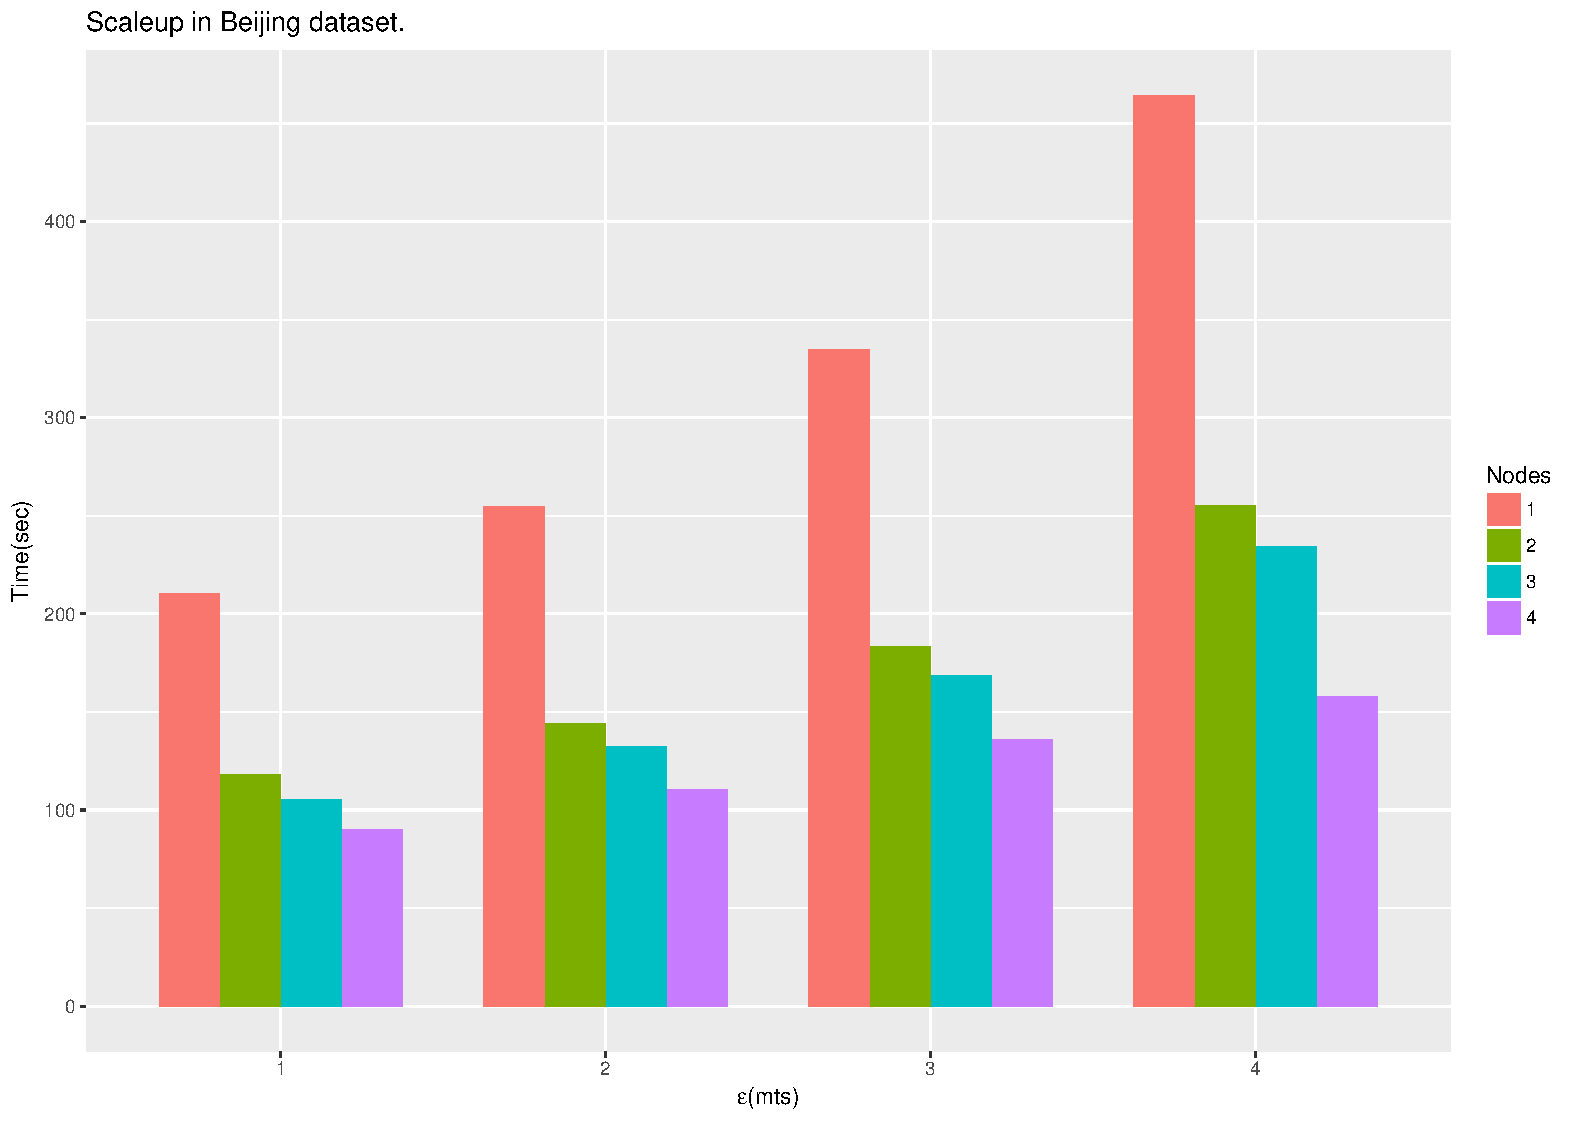
\includegraphics[height=0.85\textheight]{Figures/Ups/Beijing_Scaleup}
\end{frame}

\begin{frame}{Speedup}
  \centering
  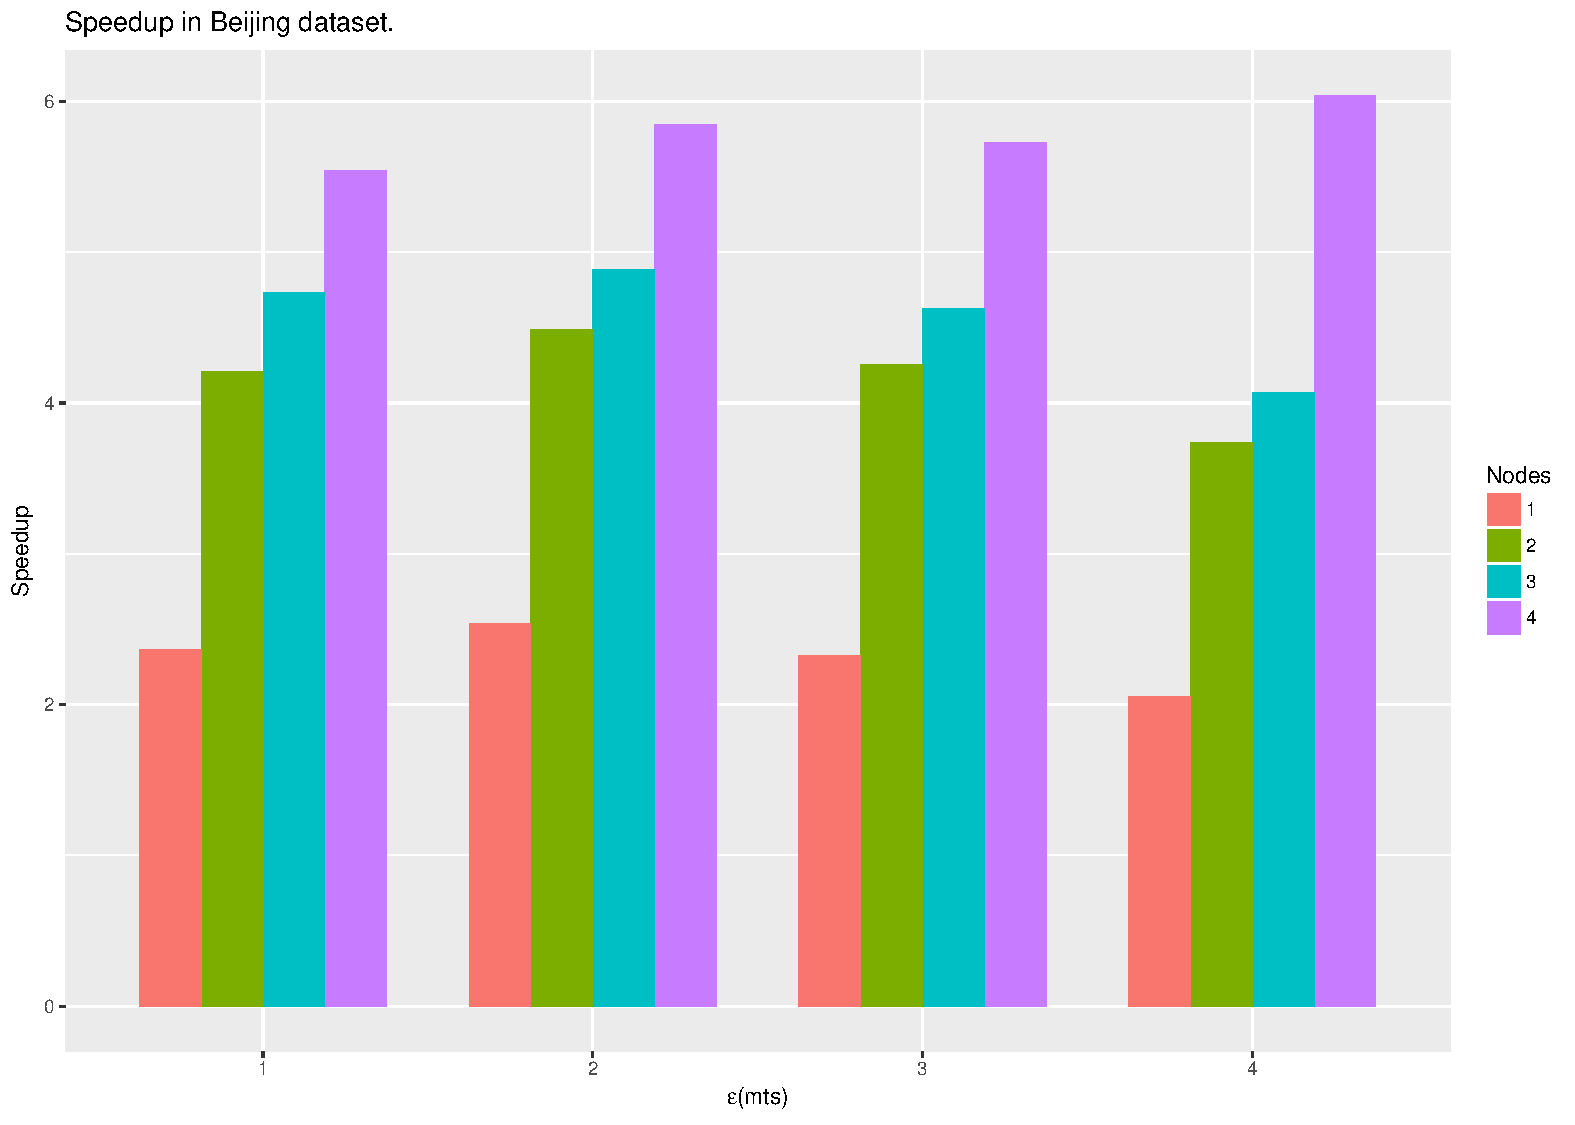
\includegraphics[height=0.85\textheight]{Figures/Ups/Beijing_Speedup}
\end{frame}

\begin{frame}{Dataset}
  \begin{itemize}
    \item \textbf{Porto} from ECML/PKDD'15 Taxi Trajectory Prediction Challenge\footnote{\tiny \url{http://tinyurl.com/zzbtlt9}}.
    \begin{itemize}
     \item A complete year (from 01/07/2013 to 30/06/2014).
     \item Trajectories for all the 442 taxis running in the city of Porto, in Portugal.
     \item $\approx$17.7 million points (no duplicates).
    \end{itemize}
  \end{itemize}
\end{frame}

\begin{frame}{Porto dataset}
  \centering
  \includegraphics[height=0.85\textheight]{Figures/porto.png}
\end{frame}

\begin{frame}{Setup}
  \begin{itemize}
    \item 4-node cluster at DBLab.
    \item Processors: 8-core Intel(R) Xeon(R) CPU E3-1230 V2 @ 3.30GHz
    \item RAM: 15.5 GB.
    \item Centos 6.8, Simba/Spark 1.6.3.
  \end{itemize}
\end{frame}

\begin{frame}{Execution time}
  \centering
  \href{http://www.cs.ucr.edu/~acald013/public/Porto_PBFE_N1M-16M_E2-10_animation.gif}{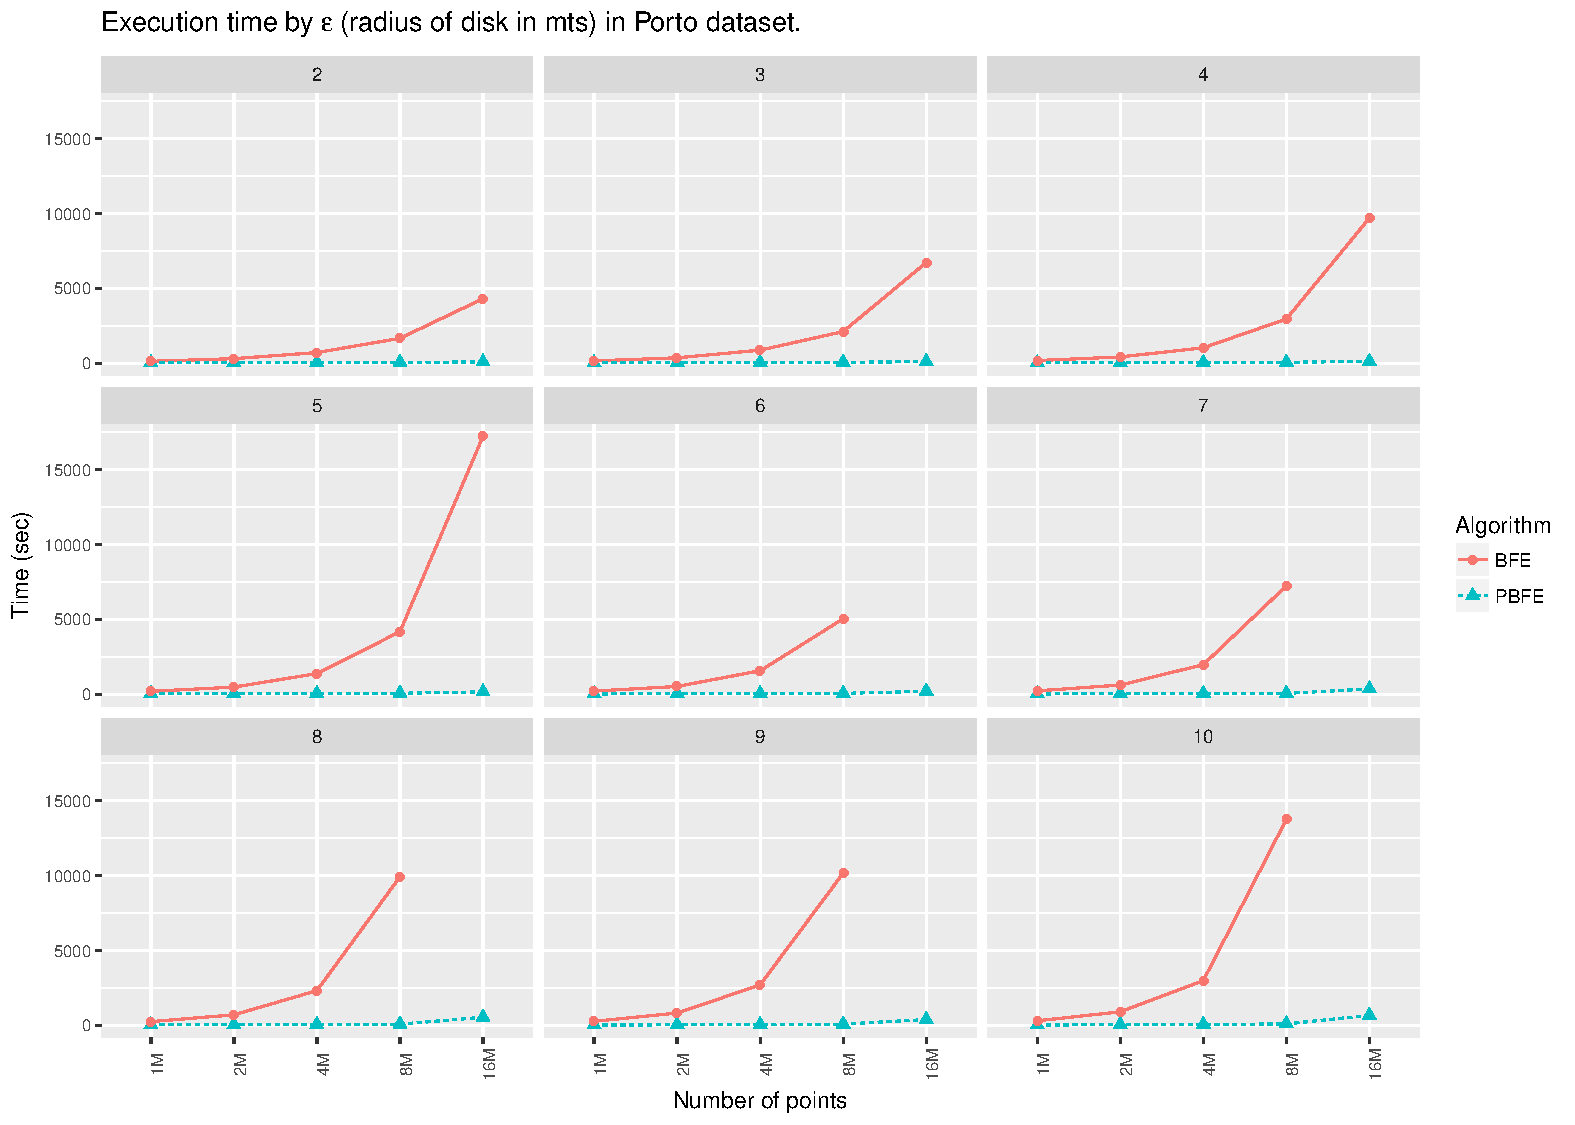
\includegraphics[width=0.88\textwidth]{Figures/Porto_PBFE_N1M-16M_E2-10}}
\end{frame}

\begin{frame}{Scaleup}
  \centering
  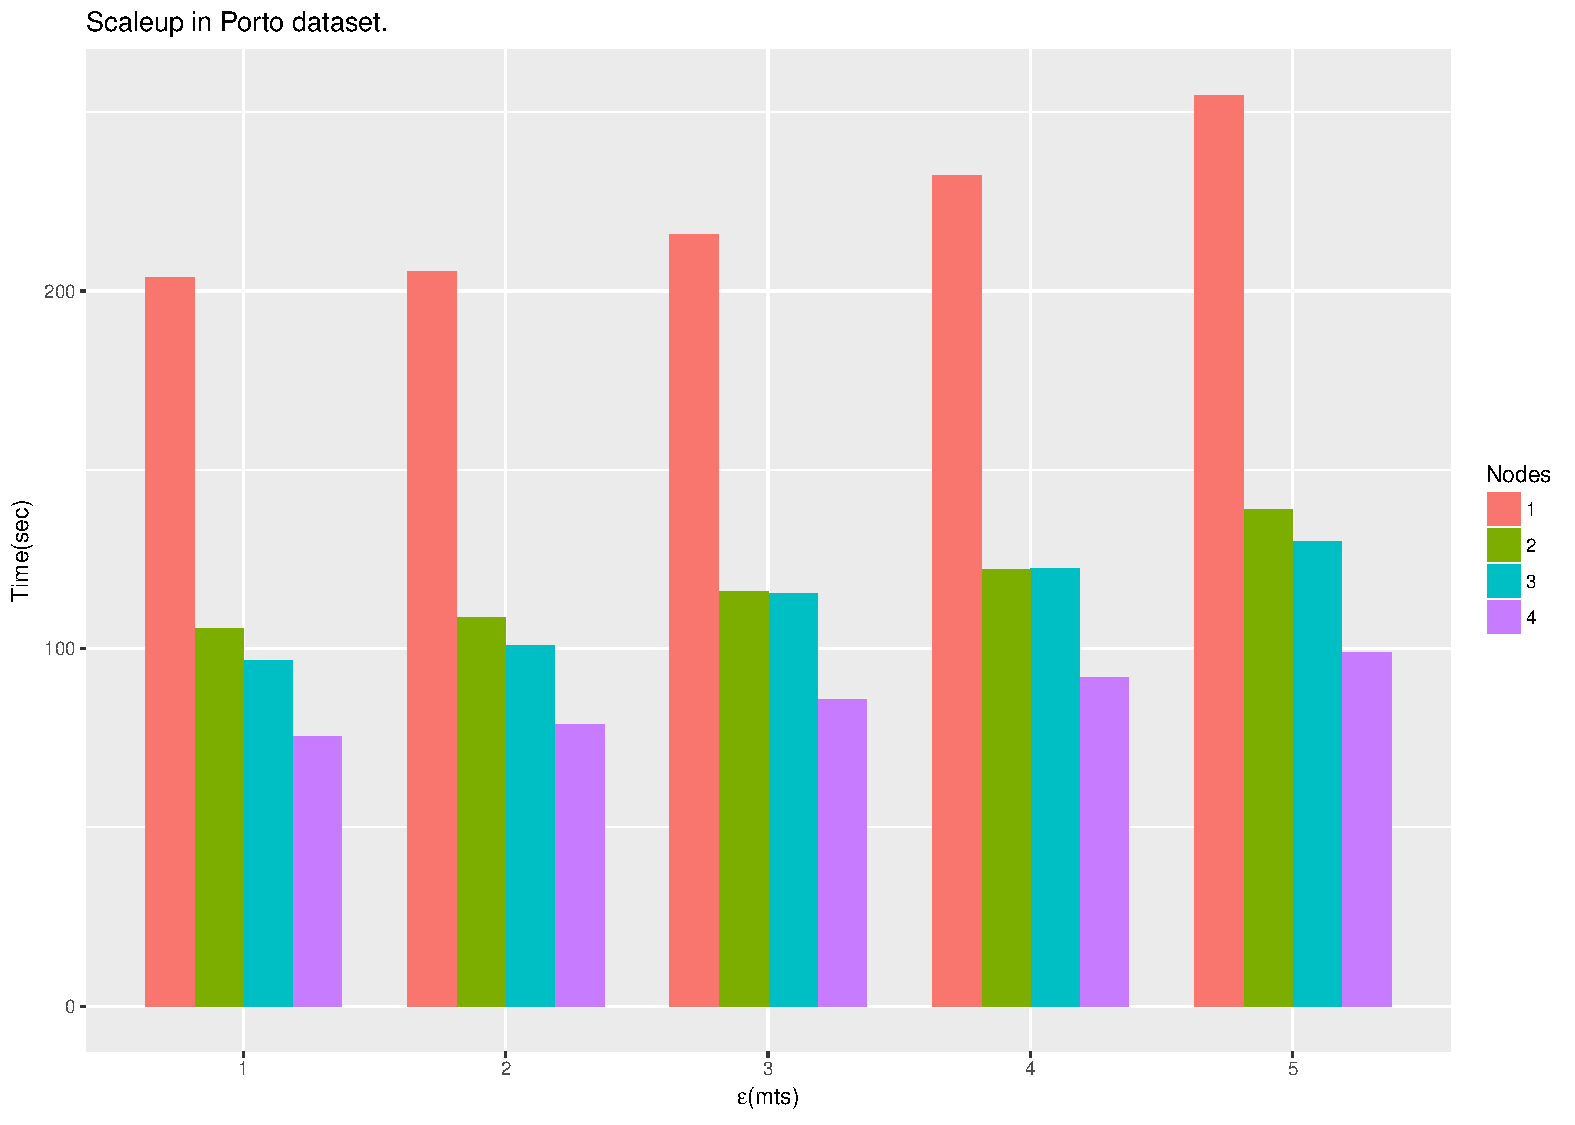
\includegraphics[height=0.85\textheight]{Figures/Ups/Porto_Scaleup}
\end{frame}

\begin{frame}{Speedup}
  \centering
  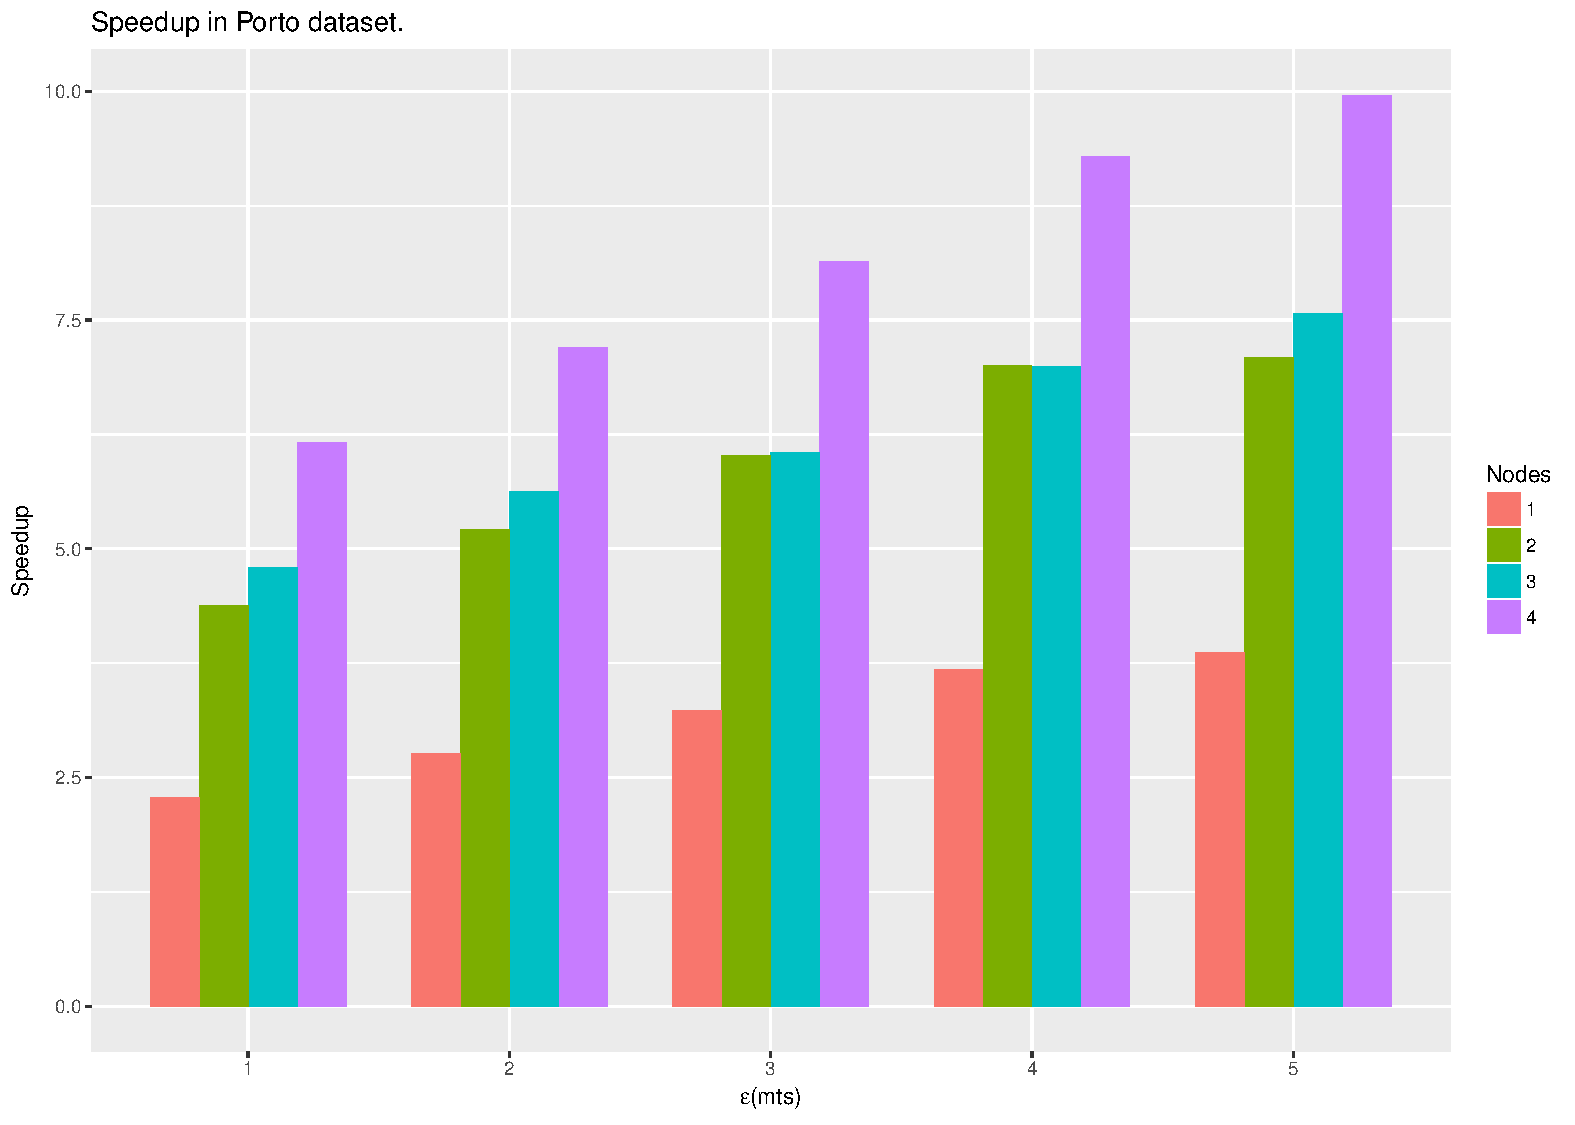
\includegraphics[height=0.85\textheight]{Figures/Ups/Porto_Speedup}
\end{frame}

\begin{frame}{Dataset}
  \begin{itemize}
    \item \textbf{Cologne} from the SUMO (Simulation of Urbar MObility) project\footnote{\tiny \url{https://tinyurl.com/l9lbw6b}}.
    \begin{itemize}
     \item Simulation scenario describing a whole-day traffic in the city of Cologne (Germany).
     \item Data demand based on traveling habits and infrastructure (TAPAS system).
     \item $\approx$70 million points (no duplicates).
    \end{itemize}
  \end{itemize}
\end{frame}

\begin{frame}{Cologne dataset}
  \centering
  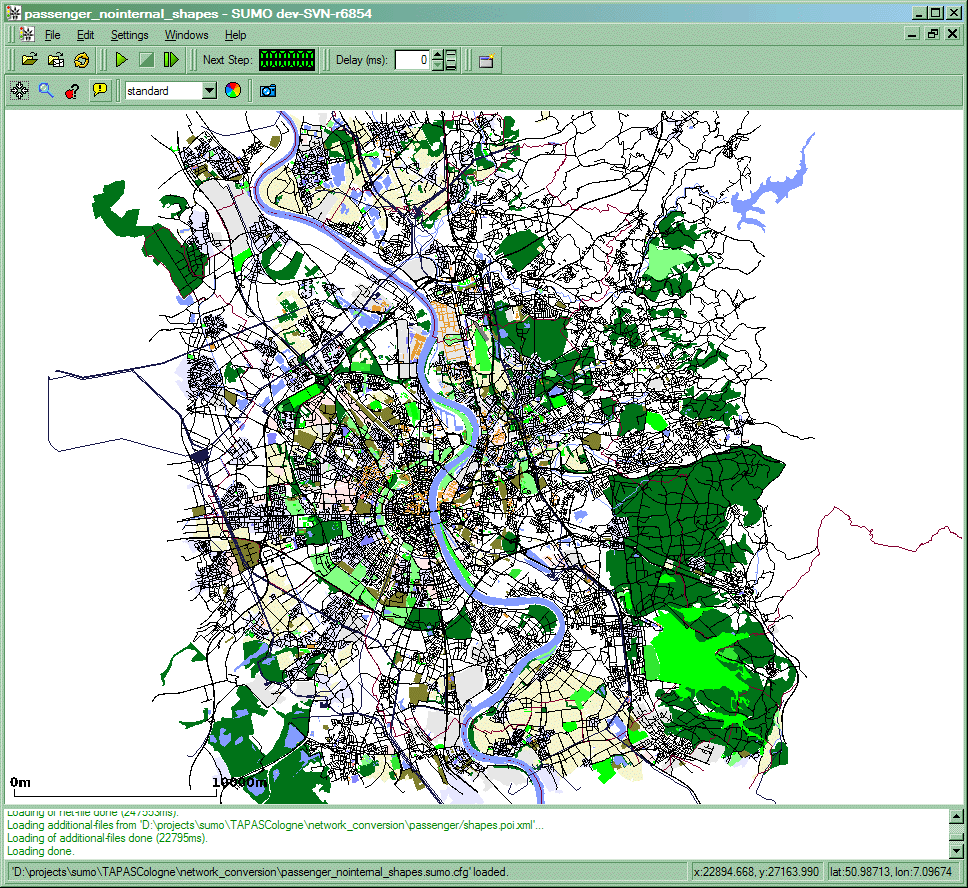
\includegraphics[height=0.85\textheight]{Figures/cologne.png}
\end{frame}

\begin{frame}{Setup}
  \begin{itemize}
    \item 4-node cluster at DBLab.
    \item Processors: 8-core Intel(R) Xeon(R) CPU E3-1230 V2 @ 3.30GHz
    \item RAM: 15.5 GB.
    \item Centos 6.8, Simba/Spark 1.6.3.
  \end{itemize}
\end{frame}

\begin{frame}{Execution time}
  \centering
  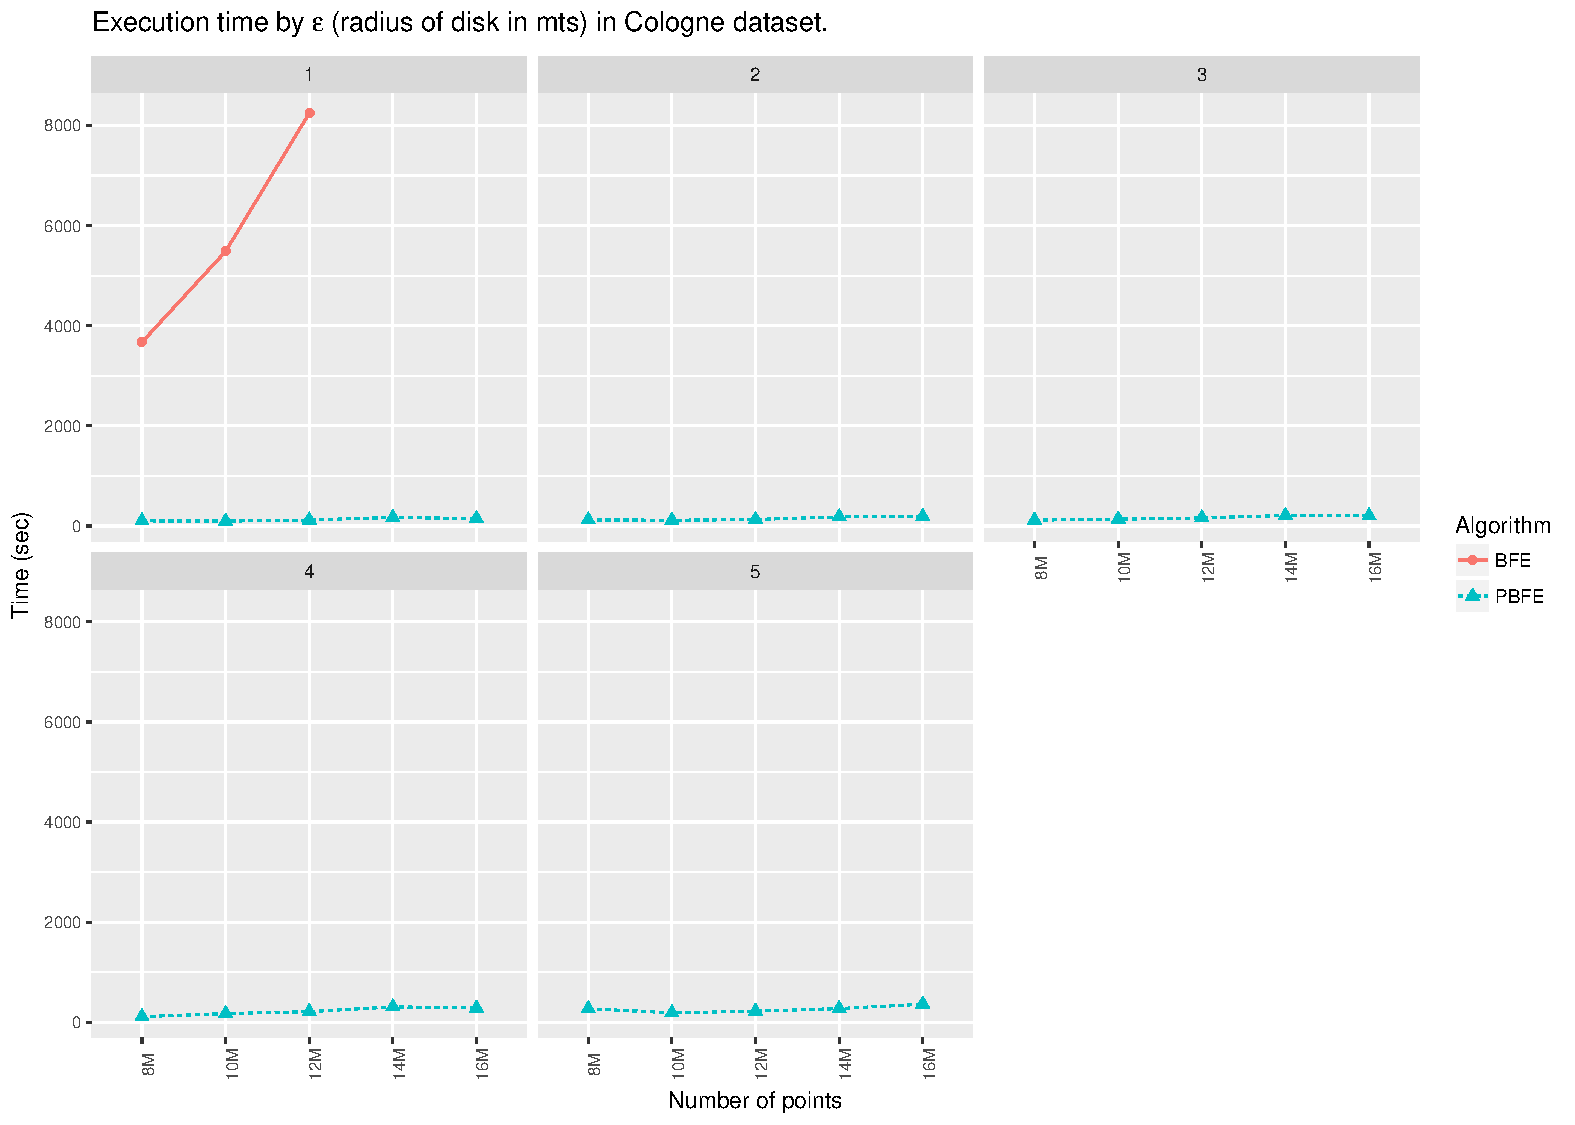
\includegraphics[width=0.88\textwidth]{Figures/Cologne_N8M-16M_E1-5}
\end{frame}

\begin{frame}{Scaleup}
  \centering
  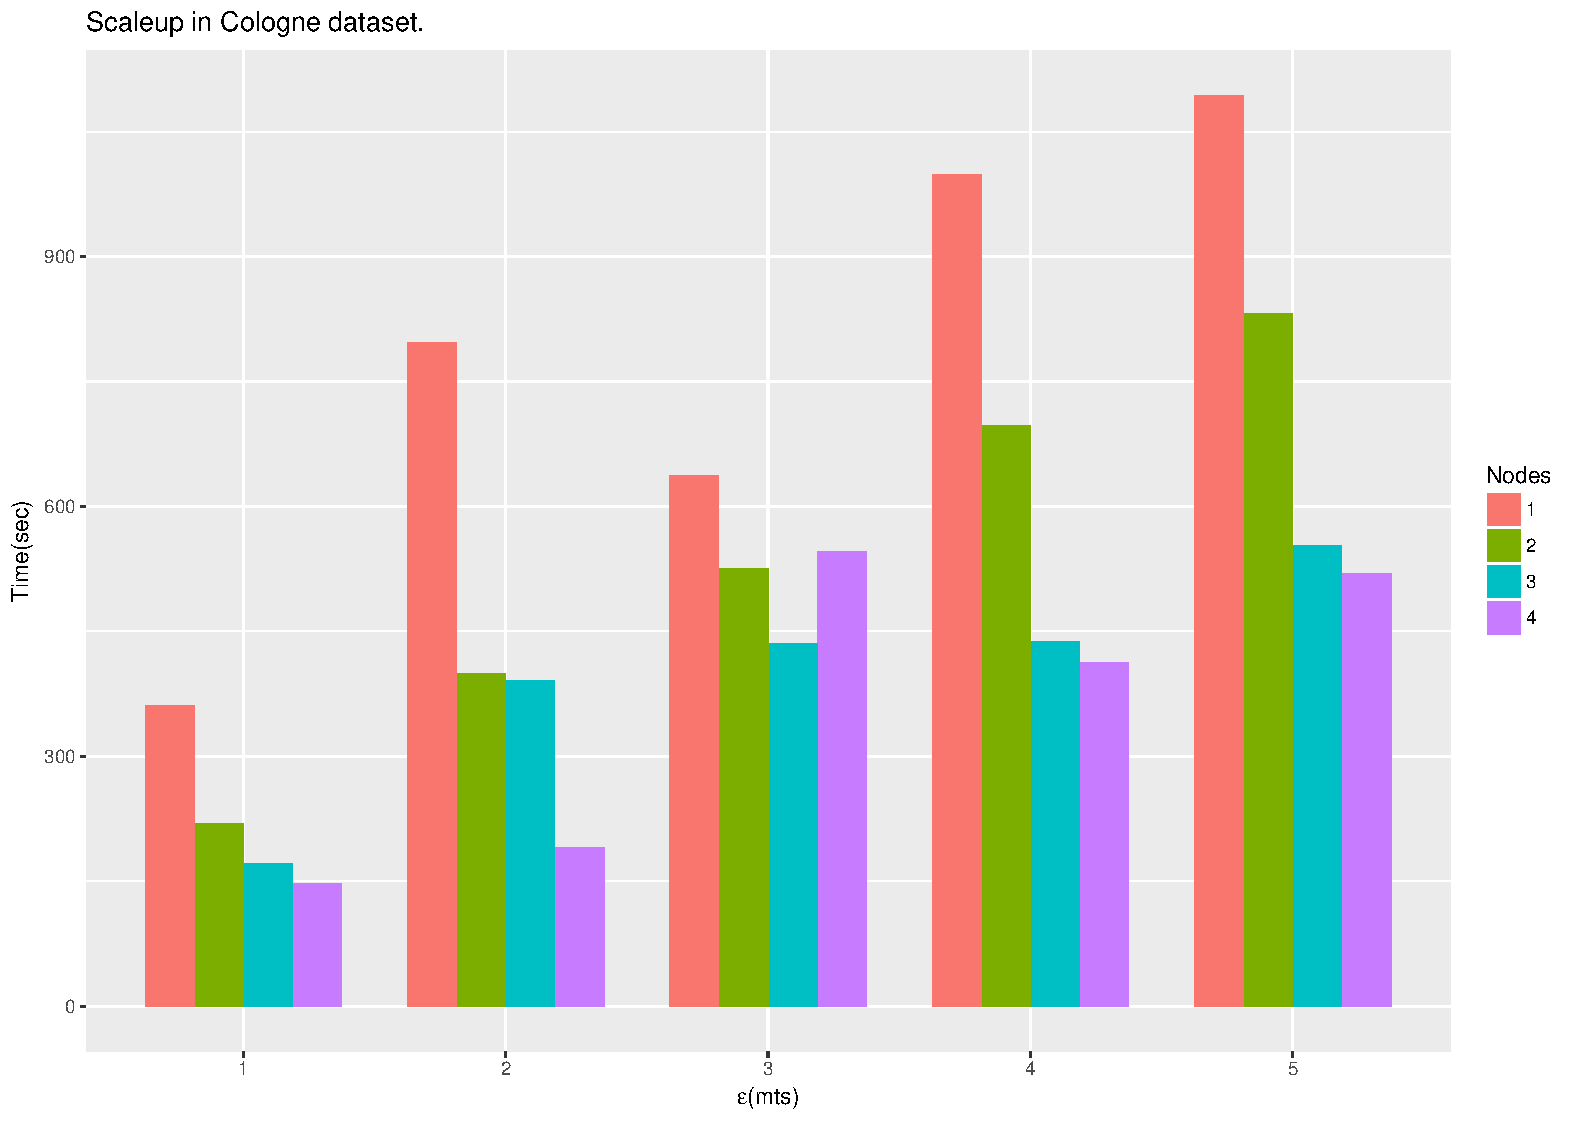
\includegraphics[height=0.85\textheight]{Figures/Ups/Cologne_Scaleup}
\end{frame}

\begin{frame}{Speedup}
  \centering
  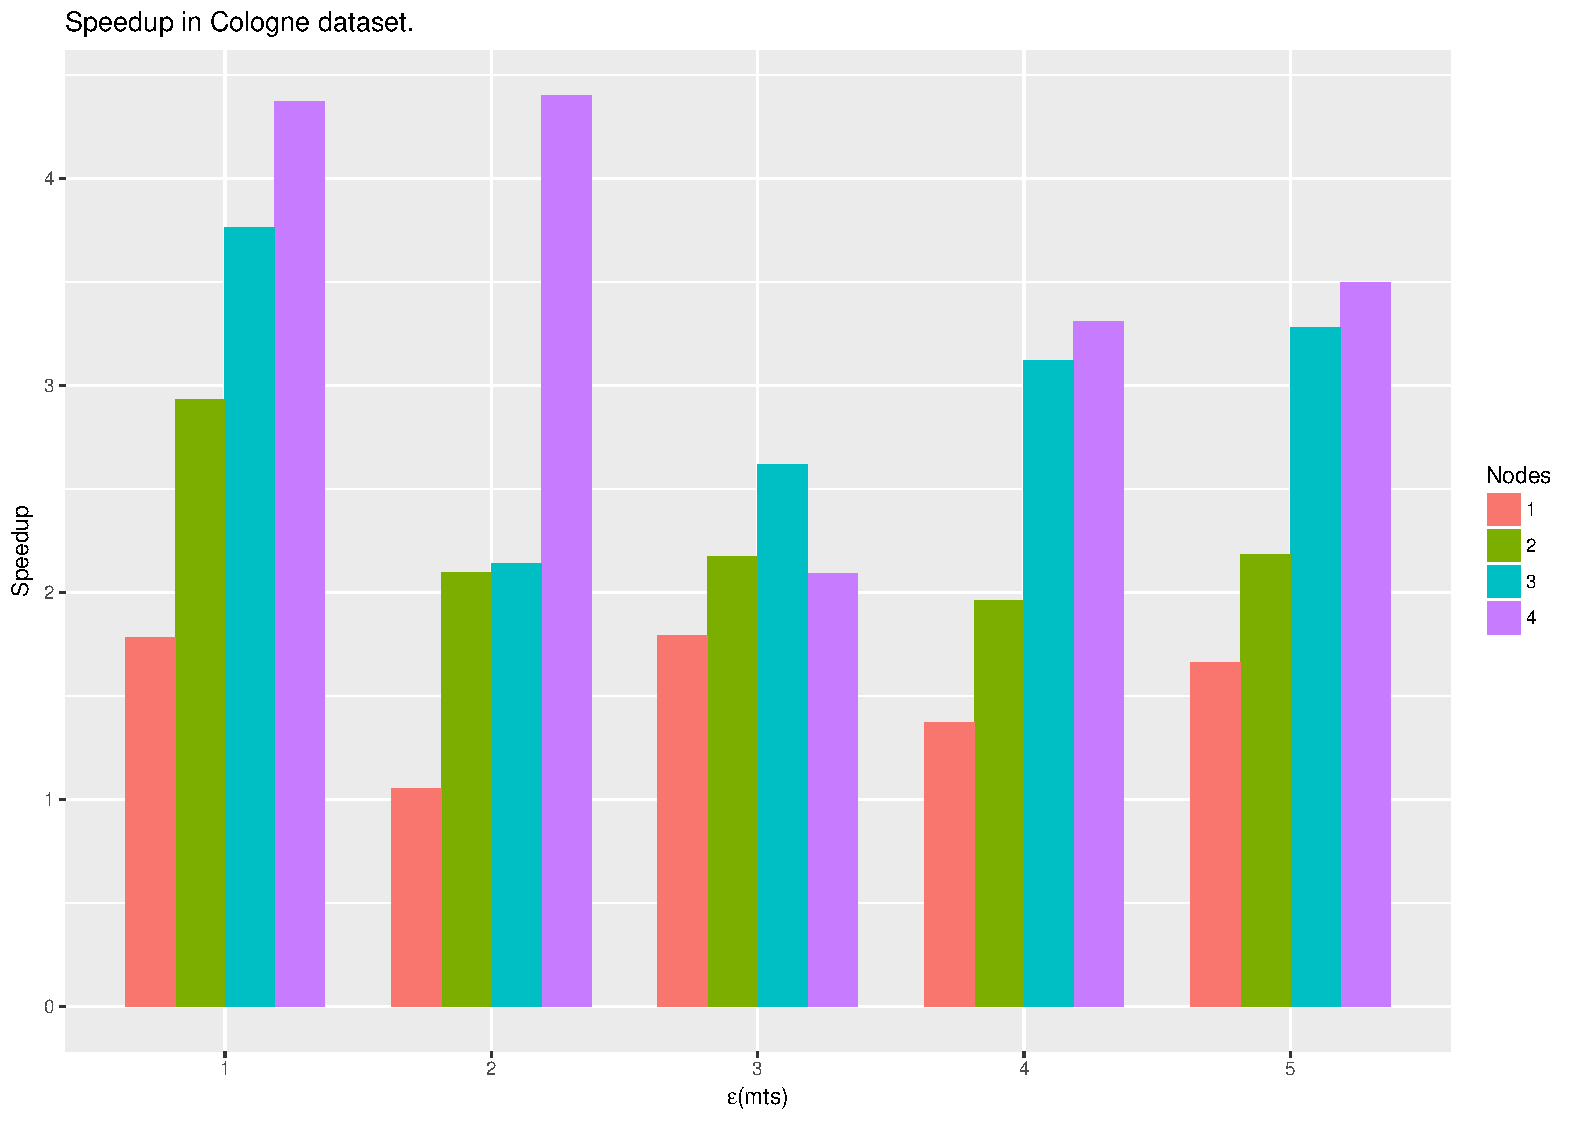
\includegraphics[height=0.85\textheight]{Figures/Ups/Cologne_Speedup}
\end{frame}

\section{Finding maximal disks}

\subsection{Implementation}

\begin{frame}{Finding maximal disks}
  \begin{itemize}
   \item The first stage of BFE finds all possible disk locations for each pair of ``close enough'' points... 
   \item This candidate set still have redundant and under-the-threshold ($\mu$) disks...
   \item BFE uses a simple approach to filter the disks but it can be costly ($O(n^2)$)
  \end{itemize}
\end{frame}

\begin{frame}{Finding maximal disks}
  \centering \includegraphics[width=\textwidth]{Figures/filter/f01.png}
\end{frame}
\begin{frame}[noframenumbering]{Finding maximal disks}
  \centering \includegraphics[width=\textwidth]{Figures/filter/f02.png}
\end{frame}
\begin{frame}[noframenumbering]{Finding maximal disks}
  \centering \includegraphics[width=\textwidth]{Figures/filter/f03.png}
\end{frame}
\begin{frame}[noframenumbering]{Finding maximal disks}
  \centering \href{http://www.cs.ucr.edu/~acald013/public/maps/gallery/pruning.html}{\includegraphics[width=\textwidth]{Figures/filter/f04.png}}
\end{frame}

\begin{frame}{Number of disks can be huge...}
  \begin{minipage}{.5\textwidth}
    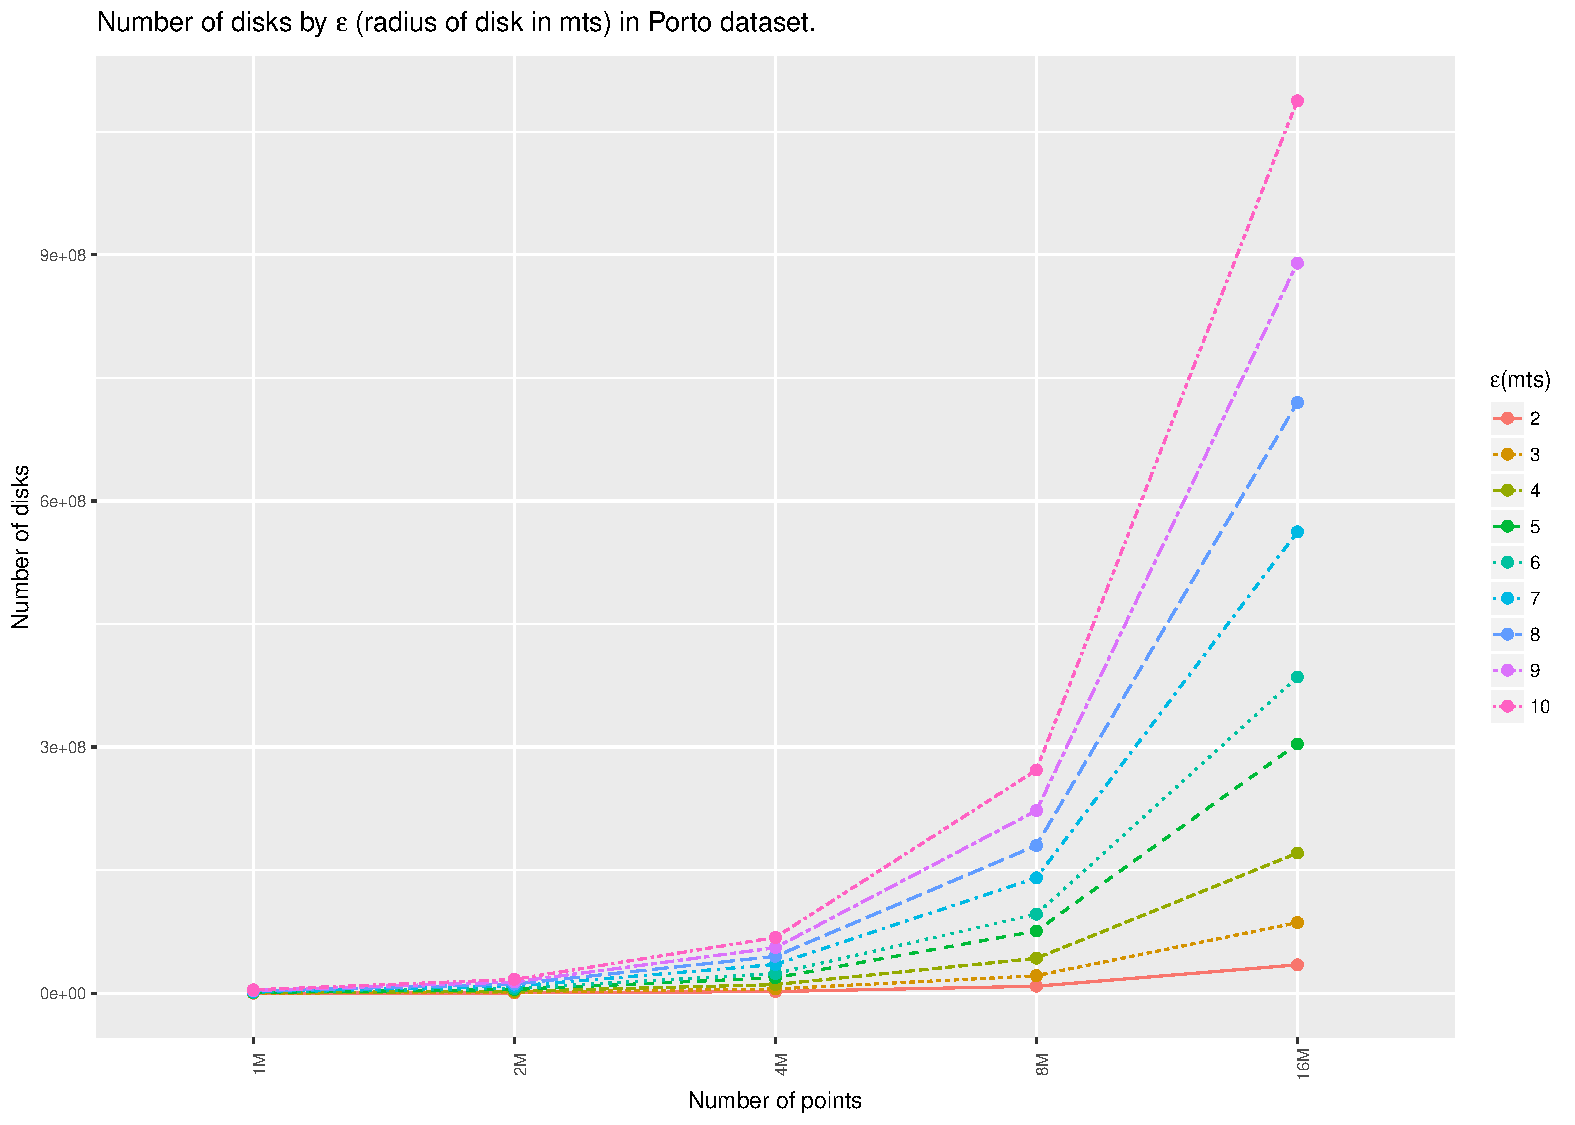
\includegraphics[width=\textwidth]{Figures/ndisks/porto}
  \end{minipage}\begin{minipage}{.5\textwidth}
    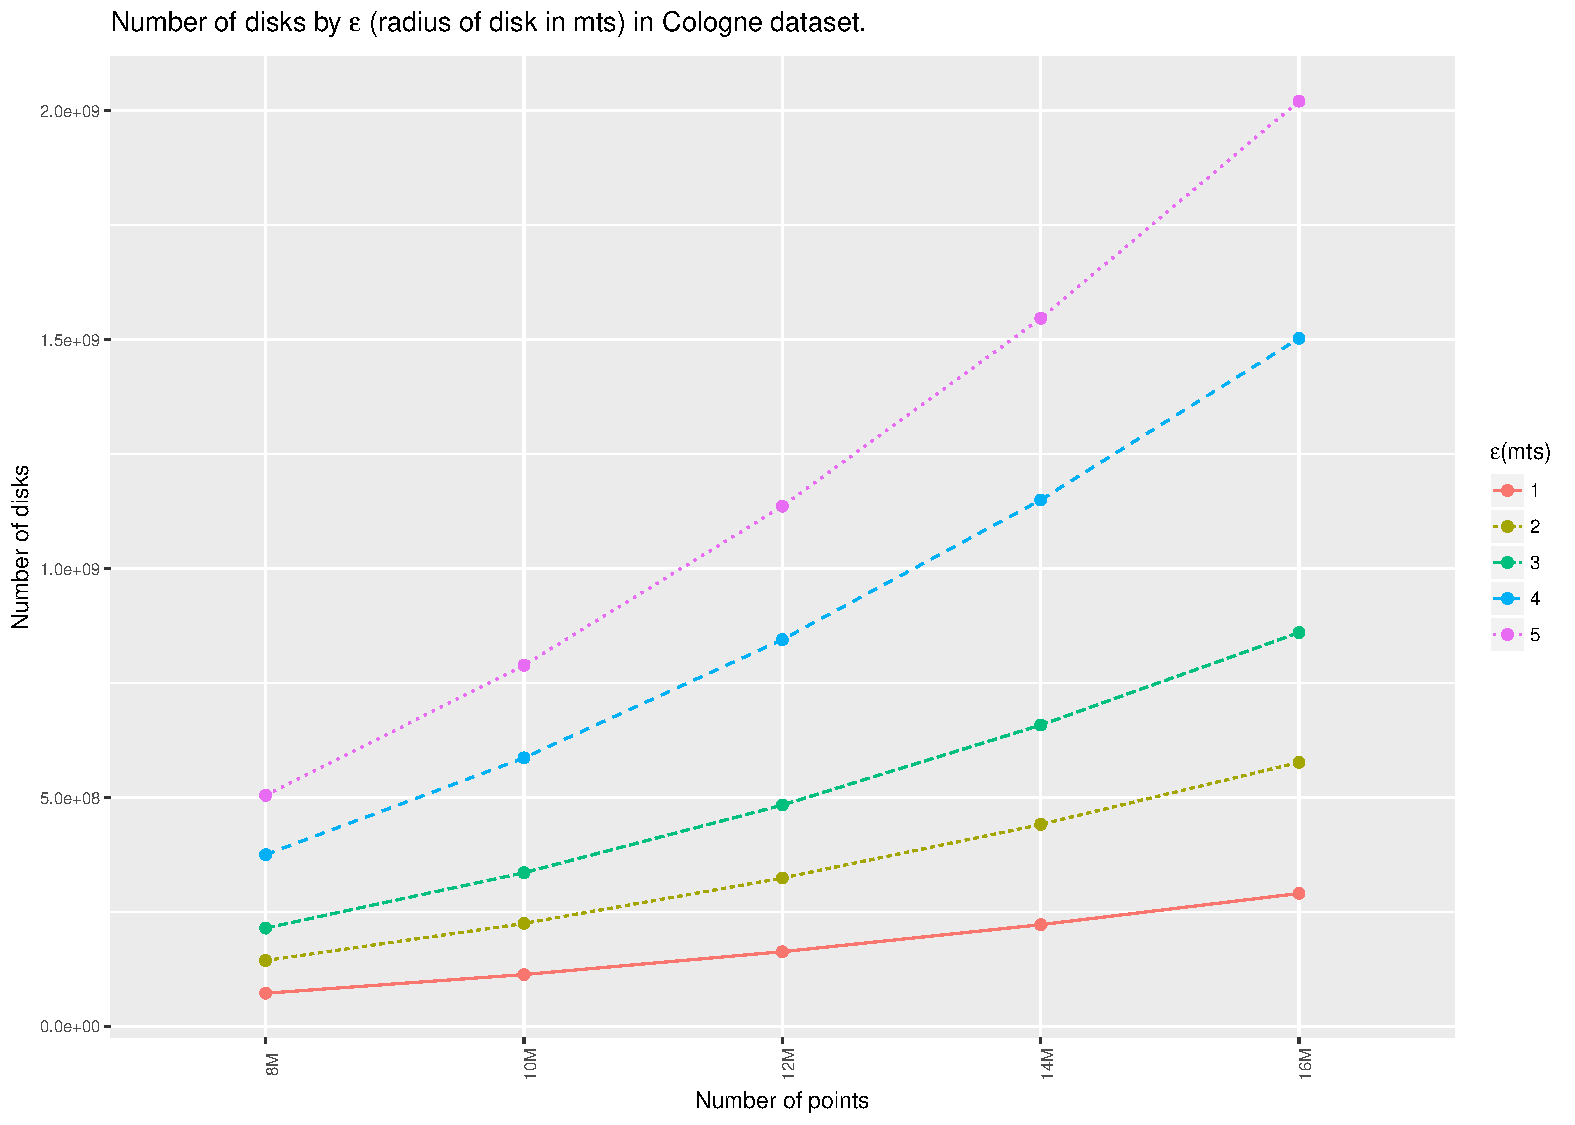
\includegraphics[width=\textwidth]{Figures/ndisks/cologne}
  \end{minipage}
\end{frame}

\begin{frame}{A Frequent/Closed/Maximal pattern example...}
	Suppose a database $D$ contains 4 transactions:
	$$ D = \{ \langle a_1,a_2, ... , a_{100} \rangle; \langle a_1,a_2, ... , a_{100} \rangle; \langle a_{20},a_{21}, ... , a_{80} \rangle; \langle a_{40},a_{41}, ... , a_{60} \rangle \} $$
	With $min\_sup=2$:
	\begin{itemize}
		\item F = $\approx 1.27 * 10^{30}$
		\item C = $\{ \{ a_1,a_2, ... , a_{100} : 2 \};\{ a_{20},a_{21}, ... , a_{80} : 3 \};\{ a_{40},a_{41}, ... , a_{60} : 4 \} \}$
		\item M = $\{ \{ a_1,a_2, ... , a_{100} : 2 \} \}$
	\end{itemize}
\end{frame}

\begin{frame}{Finding maximal disks using Maximal Pattern algorithms}
  \begin{itemize}
   \item Points enclosed by disks become transactions...
   \item Apply well-know algorithms (LCM in this case)...
   \item Filter patterns with length less than $\mu$.
  \end{itemize}
\end{frame}

\subsection{Experiments}

\begin{frame}{Setup}
  \begin{itemize}
    \item 4-node cluster at DBLab.
    \item Processors: 8-core Intel(R) Xeon(R) CPU E3-1230 V2 @ 3.30GHz
    \item RAM: 15.5 GB.
    \item Centos 6.8, Simba/Spark 1.6.3.
  \end{itemize}
\end{frame}

\begin{frame}{Beijing - Execution time}
  \centering 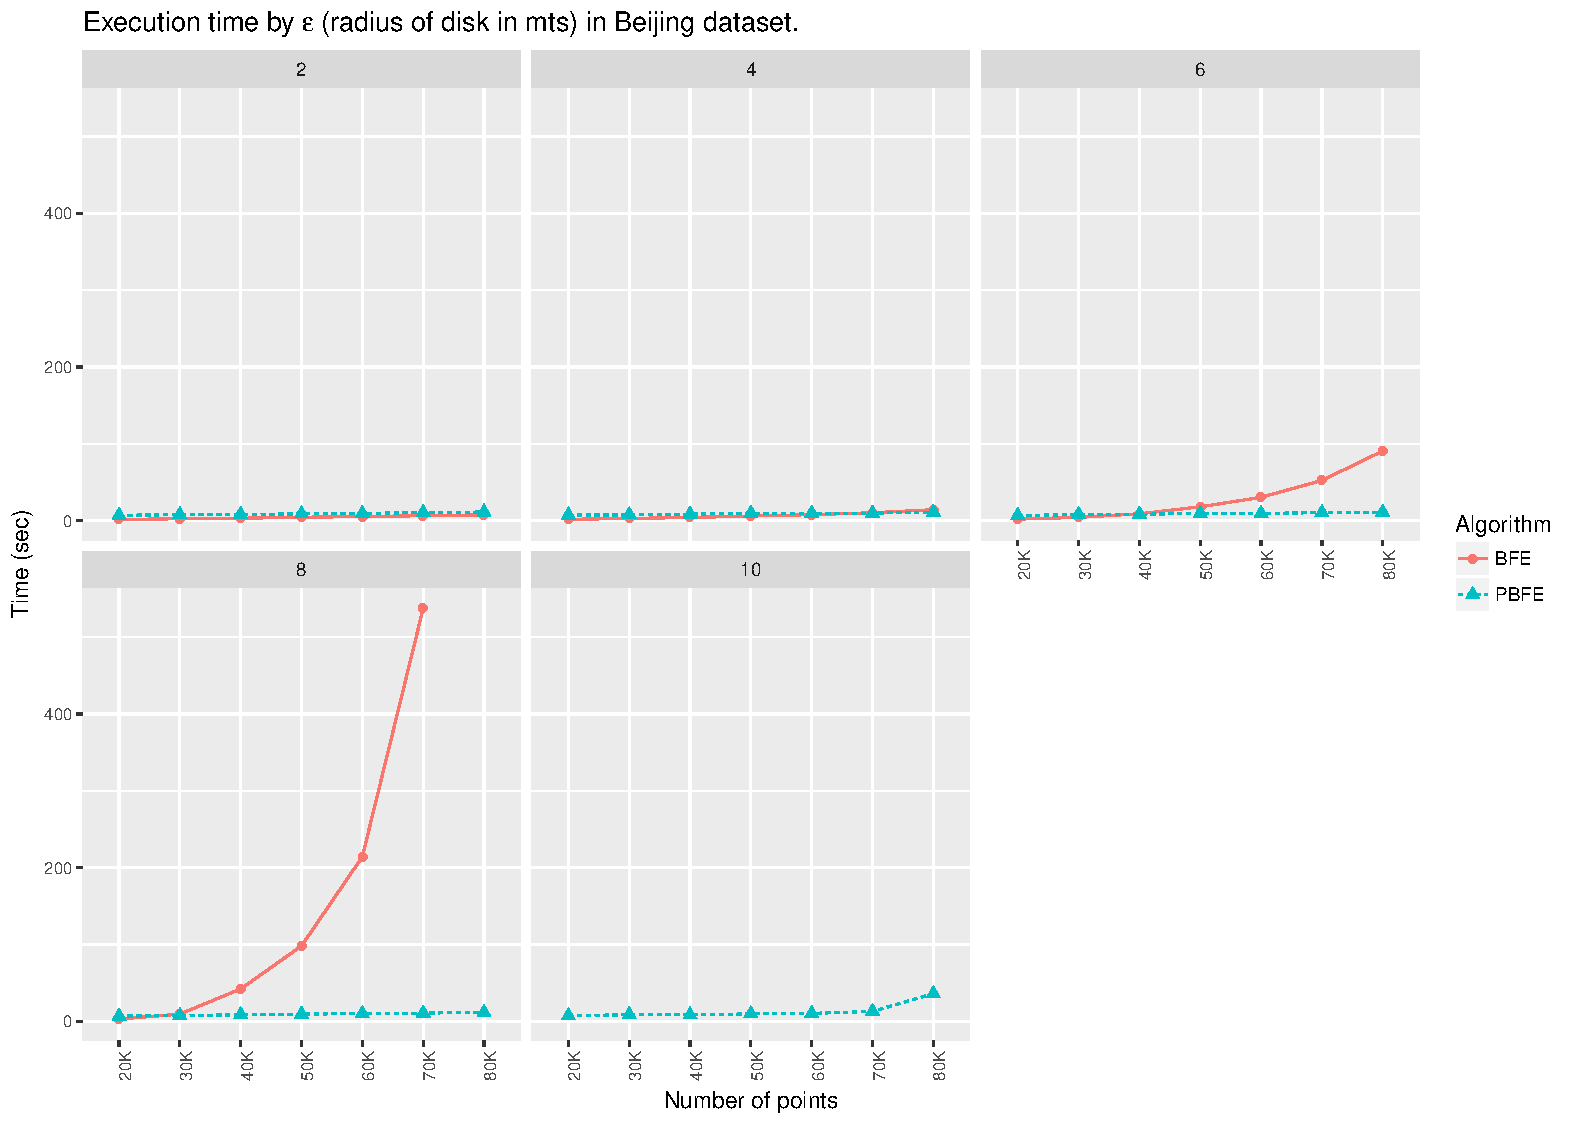
\includegraphics[height=0.85\textheight]{Figures/Maximal/beijing.pdf}
\end{frame}

\begin{frame}{Porto - Execution time}
  \centering \includegraphics[height=0.85\textheight]{Figures/Maximal/porto.pdf}
\end{frame}

\section{Conclusions and future work}

\begin{frame}{Conclusions}
  \begin{itemize}\pause
   \item An implementation of a parallel method to detect a maximal set of disks for the BFE algorithm has been presented.\pause
   \item The finding of a candidate set of disk proves to be scalable and reliable.\pause
   \item Execution time improves up to 3 orders of magnitude compared to the sequential code.\pause
   \item Good behavior of Scaleup and Speedup metrics.\pause
   \item Promising performance for the detection of maximal set of disks.\pause
  \end{itemize}
\end{frame}

\begin{frame}{Future work}
  \begin{itemize}\pause
   \item Work on a parallel strategy to join the sets of valid disks between time intervals.\pause
   \item Explore other partition strategies for finding maximal set of disks as alternative to the local-global approach.\pause
   \item Test the approach with other spatio-temporal patterns.\pause
  \end{itemize}
\end{frame}

\subsection*{Thanks...}

\begin{frame}{}
  \centering
  \huge Thank you!!! \\
  \vspace{2cm}
  \large Do you have any question?
\end{frame}

\end{document}